\chapter{Quality of experience evaluation}
\label{cha:eval}

In this section, we illustrate how we set up a \textbf{testbed} with ComNetsEmu to evaluate the performance of \textbf{low-latency adaptive bitrate live streaming} and the results that we obtained. Some important metrics are extracted and plotted to highlight the issues of current streaming technologies in low-latency scenarios. The results of the evaluation will be the basis for some proposed improvements that we believe produce an overall better \textbf{quality of experience}.


\section{Testbed setup}
\label{sec:eval/testbed}

The testbed for evaluating the quality of experience (QoE) of existing live streaming solutions, such as HLS and DASH, was built with ComNetsEmu. The project was published as an open source project at \url{https://github.com/matteocontrini/live-streaming-testbed}.

The general architecture of the testbed is shown in Figure X. The topology of the emulated network consists of three hosts and two switches. The link between the two switches (S1 and S2) represents an unreliable network such as an Internet access network. When the emulation is run, a series of experiments with different configurations are run, and the link parameters are changed. For example, the bandwidth is varied to emulate a real network with oscillating bandwidth.

The three hosts contain Docker applications for a live streaming setup. More in detail:

\begin{itemize}
    \item \texttt{H3} hosts a script that performs the \textbf{packaging of a live stream} in both HLS and DASH formats. It runs an \ffmpeg{} command that simulates a live stream, taking an MP4 file as input. The output of this application, called \textit{live source}, are manifest and playlist files for both HLS and DASH, and the corresponding video and audio segments.
    \item \texttt{H2} acts as an \textbf{HTTP CDN server} for static files. It serves the files produced by the live source over HTTP/1.1, HTTP/2 and HTTP/3 through the \texttt{h2o} web server. It also takes care of provisioning the public key certificates that are required for HTTPS.
    \item \texttt{H1}, on the other side of the main network link, is the client. It consists of a frontend application containing a \textbf{video player} that plays the live video stream generated by the server. The frontend application also takes care of collecting several metrics from the player and transmit them to a Node.js backend application. The frontend application runs in a \textbf{Chromium headless} instance, which is started by the backend application through the Puppeteer library.
\end{itemize}

% TODO: diagram

To start the emulation through ComNetsEmu, one first needs to clone the testbed source code and prepare the MP4 file for the live source, as we will see in detail in the next section. Then, a Vagrant session should be started:

\begin{minted}[frame=single]{bash}
vagrant up
vagrant ssh
\end{minted}

Finally, after building the Docker images, the emulation can be started. The project source code contains scripts to run these commands more easily.

\begin{minted}[frame=single]{bash}
cd live-source && docker build -t live-source .
cd ../cdn && docker build -t cdn .
cd ../client && docker build -t client .
cd .. && sudo python3 topology.py
\end{minted}

Before going into the details of how the specific components were developed, it should be noted that the default Vagrant configuration for ComNetsEmu (contained in a file known as \texttt{Vagrantfile}) does not work when the machine architecture is ARM. This is especially problematic on newer laptops that use Apple Silicon hardware, such as the M1 and M2 chips.

To solve this problem, two changes must be applied to ComNetsEmu's \texttt{Vagrantfile}. First, the Vagrant box (the operating system image) must be changed to an image that is built for ARM architectures. Then, since x86 virtualization software like VirtualBox cannot be used on ARM systems, a new virtual machine provider must be added. In practice, for Mac systems, this means enabling Parallels Desktop as a virtual machine provider. Figure \ref{fig:vagrantfile} shows how the \texttt{Vagrantfile} of ComNetsEmu was changed.

\begin{figure}
    \centering
    \begin{minted}[frame=single,linenos,fontsize=\small]{diff}
diff --git a/Vagrantfile b/Vagrantfile
index 0f07076..a21824f 100644
--- a/Vagrantfile
+++ b/Vagrantfile
@@ -20,6 +20,8 @@ VM_NAME = "ubuntu-20.04-comnetsemu"
 # When using libvirt as the provider, use this box, bento boxes do not support...
 BOX_LIBVIRT = "generic/ubuntu2004"

+BOX_PARALLELS = "jeffnoxon/ubuntu-20.04-arm64"
+
 ######################
 #  Provision Script  #
 ######################
@@ -105,6 +107,14 @@ Vagrant.configure("2") do |config|
     # Sync ./ to home directory of vagrant to simplify the install script
     comnetsemu.vm.synced_folder ".", "/vagrant", disabled: true
     comnetsemu.vm.synced_folder ".", "/home/vagrant/comnetsemu"
+
+    # Parallels Desktop
+    config.vm.provider "parallels" do |prl, override|
+      override.vm.box = BOX_PARALLELS
+      prl.name = VM_NAME
+      prl.cpus = CPUS
+      prl.memory = RAM
+    end

     # For Virtualbox provider
     comnetsemu.vm.provider "virtualbox" do |vb|
    \end{minted}
    \caption{Caption}
    \label{fig:vagrantfile}
\end{figure}


\subsection{Live stream generation and packaging}
\label{sec:eval/testbed/packaging}

There are multiple ways to simulate a live video stream without having an actual live video source such as a camera. Although there exist many streaming servers that handle video ingestion, transcoding and packaging, we chose to implement a simpler solution based on \ffmpeg{} and a static input video file.

Moreover, since the source of the live stream is not dynamic, we decided to encode the video and audio renditions beforehand. The renditions are then packaged as live streams each time the emulation is run, as if they were ingested and transcoded live. This solution makes the test setup much lighter in terms of required computational resources.

When encoding the video renditions, we chose the following bitrate ladder. All video renditions are encoded with H.264 at 25 fps with a keyframe/I-frame interval of 2 seconds and a constant bitrate.

\begin{itemize}
    \item \texttt{1280x720} at 3.5 Mbps;
    \item \texttt{960x540} at 2.5 Mbps;
    \item \texttt{640x360} at 1.5 Mbps;
    \item \texttt{480x720} at 0.8 Mbps.
\end{itemize}

The audio is instead encoded with \texttt{AAC-LC} at 128 kbps. There are of course many more possible configurations, but the above is a common configuration that gives good quality results.\cite{ozer}

The \ffmpeg{} command that was used to produce the renditions is similar to the following:

\begin{minted}[frame=single,fontsize=\small]{bash}
ffmpeg -i $INPUT \
  -c:v libx264 -pix_fmt yuv420p -preset veryfast -r 25 \
  -g 50 -keyint_min 50 -sc_threshold 0 \
  -force_key_frames 'expr:gte(t,n_forced*2)' -refs 1 \
  -c:a libfdk_aac -ac 2 -b:a 128k \
  -map 0:a:0 -map 0:v:0 -map 0:v:0 -map 0:v:0 -map 0:v:0 \
  -s:v:0 1280x720 -b:v:0 3500k -bufsize:v:0 3500k -minrate:v:0 3500k -maxrate:v:0 3500k \
  -s:v:1 960x540 -b:v:1 2500k -bufsize:v:1 2500k -minrate:v:1 2500k -maxrate:v:1 2500k \
  -s:v:2 640x360 -b:v:2 1500k -bufsize:v:2 1500k -minrate:v:2 1500k -maxrate:v:2 1500k \
  -s:v:3 480x270 -b:v:3 800k -bufsize:v:3 800k -minrate:v:3 800k -maxrate:v:3 800k \
  abr.mp4
\end{minted}

In detail, the meaning of the options is as follows:

\begin{itemize}
    \item \texttt{-i} specifies the input media file, which can be in any format supported by \ffmpeg{};
    \item \texttt{-c:v} specifies the video codec, in this case \texttt{libx264}, the library that implements x264, a popular open source software-based H.264 encoder;
    \item \texttt{-pix\_fmt} defines the pixel format. A value of \texttt{yuv420p} means that the pixels are encoded with Y'CbCr 4:2:0 chroma subsampling;
    \item \texttt{-preset} specifies a set of configuration options that influence the encoding speed. Research has shown that \texttt{veryfast} is a good trade-off between speed and quality;\cite{ozer}
    \item \texttt{-r} sets the \textit{frames per second} (fps) value, in this case 25;
    \item \texttt{-g} and \texttt{-keyint\_min} tell the encoder the maximum and minimum GOP size in frames, that is, the minimum and maximum interval between key frames (I-frames);
    \item \texttt{-sc\_threshold} adjusts the scene cut detection, an algorithm that analyzes the difference between frames to determine whether a new I-frame should be inserted. Setting the parameter to 0 means that the scene cuts detection is disabled. This is a common choice when encoding for streaming, since I-frames are very expensive compared to other frame types.\cite{ozer}
    \item \texttt{-force\_key\_frames} forces a key frame when the given expression evaluates to \texttt{true} at the current frame. This option is required because \texttt{x264} does not allow setting \texttt{-keyint\_min} to a value greater than \texttt{keyint/2+1}, and clips the value if it is larger.\footnote{\url{https://github.com/mirror/x264/blob/b093bbe7d9bc642c8f24067cbdcc73bb43562eab/encoder/encoder.c\#L1111}} The expression \texttt{gte(t,n\_forced*2)} means that a keyframe should be forced every 2 seconds, since \texttt{t} is the time of the current frame and \texttt{n\_forced} is the number of forced frames;
    \item \texttt{-refs} specifies the number of reference frames that each inter-predicted frame can use. Research has shown that limiting the number of frames to 1 has a negligible impact on quality while reducing the encoding time;\cite{ozer}
    \item \texttt{-c:a} specifies the audio codec, in this case \texttt{libfdk\_aac}, a high quality AAC implementation by the Fraunhofer research institute.
    \item \texttt{-ac} specifies the number of audio channels, 2 in this case;
    \item \texttt{-b:a} sets the audio bitrate, which is constant (CBR) by default;
    \item \texttt{-map} is used to select which streams of the input file should be sent to the output. For example, \texttt{-map 0:a:0} takes the first audio track from the first input file and includes it in the output file. Multiple \texttt{-map} options for the same input stream have the effect of duplicating the stream. In this case, we use \texttt{-map} to create multiple video streams (one per rendition) with a single command;
    \item \texttt{-s:v} is used to scale the video to the specified resolution. In our command this option is used once per rendition to change the resolution for reach of the (duplicated) video streams;
    \item \texttt{-b:v}, \texttt{-minrate:v}, \texttt{-maxrate:v}, \texttt{-bufsize:v} set the average target bitrate, the minimum bitrate, the maximum bitrate, and the buffer size of the encoder. By setting all the options to the same value the result is a constant bitrate (CBR) video stream, which is often recommended for adaptive bitrate streaming and helps to comply with Apple HLS Authoring Specification;\cite{ozer}\cite{hlsauthoring}
\end{itemize}

The output is a single MP4 file containing multiple tracks, one per each video rendition and one for the audio, as shown in Figure \ref{fig:ffprobe_abr}.

\begin{figure}
    \centering
    \begin{minted}[frame=single,breaklines,fontsize=\footnotesize]{text}
Input #0, mov,mp4,m4a,3gp,3g2,mj2, from 'abr.mp4':
  Metadata:
    major_brand     : isom
    minor_version   : 512
    compatible_brands: isomiso2avc1mp41
    title           : Big Buck Bunny, Sunflower version
    artist          : Blender Foundation 2008, Janus Bager Kristensen 2013
    composer        : Sacha Goedegebure
    encoder         : Lavf59.31.100
    comment         : Creative Commons Attribution 3.0 - http://bbb3d.renderfarming.net
    genre           : Animation
  Duration: 00:10:34.64, start: 0.000000, bitrate: 7884 kb/s
  
  Stream #0:0[0x1](und): Audio: aac (LC) (mp4a / 0x6134706D), 48000 Hz, stereo, fltp, 128 kb/s (default)
  
  Stream #0:1[0x2](und): Video: h264 (High) (avc1 / 0x31637661), yuv420p(progressive), 1280x720 [SAR 1:1 DAR 16:9], 3238 kb/s, 25 fps, 25 tbr, 12800 tbn (default)
  
  Stream #0:2[0x3](und): Video: h264 (High) (avc1 / 0x31637661), yuv420p(progressive), 960x540 [SAR 1:1 DAR 16:9], 2341 kb/s, 25 fps, 25 tbr, 12800 tbn (default)
  
  Stream #0:3[0x4](und): Video: h264 (High) (avc1 / 0x31637661), yuv420p(progressive), 640x360 [SAR 1:1 DAR 16:9], 1409 kb/s, 25 fps, 25 tbr, 12800 tbn (default)
  
  Stream #0:4[0x5](und): Video: h264 (High) (avc1 / 0x31637661), yuv420p(progressive), 480x270 [SAR 1:1 DAR 16:9], 751 kb/s, 25 fps, 25 tbr, 12800 tbn (default)
  
    \end{minted}
    \caption{\texttt{ffprobe}'s output showing the 5 video tracks of the ABR MP4 file. Some metadata was omitted for brevity.}
    \label{fig:ffprobe_abr}
\end{figure}

As we have seen, when the emulation starts one of the applications that is run is the live source generation, or ABR packaging. This is again a \ffmpeg{} script, run inside a Docker container. The script takes the previously generated MP4 file as input and outputs \texttt{fMP4} chunks, HLS playlists, and the DASH manifest, for all the renditions.

The \ffmpeg{} command used for packaging is similar to the following:

\begin{minted}[frame=single]{bash}
ffmpeg -re -i $SOURCE \
  -map 0 -c copy \
  -utc_timing_url 'https://time.akamai.com/?iso' \
  -seg_duration 2 \
  -dash_segment_type mp4 \
  -use_template 1 -use_timeline 0 \
  -init_seg_name 'init-stream-$RepresentationID$.m4s' \
  -media_seg_name 'chunk-stream-$RepresentationID$-$Number%05d$.m4s' \
  -adaptation_sets 'id=0,streams=v id=1,streams=a' \
  -hls_playlist 1 \
  -f dash \
  $OUT_DIR/manifest.mpd
\end{minted}

Specifically, the meaning of the arguments and options is as follows.

\begin{itemize}
    \item \texttt{-re} limits the read rate so that it respects the frame rate, otherwise \ffmpeg{} would read the whole video without respecting the playback rate;
    \item \texttt{-c} with a value of \texttt{copy} tells \ffmpeg{} to copy the input streams without re-encoding, since we have already encoded them previously;
    \item \texttt{-utc\_timing\_url} defines the URL of a web page that returns the current UTC timestamp in ISO format. This is needed by DASH on the client side for time synchronization when performing live streaming;
    \item \texttt{-seg\_duration} specifies the duration of each segment or fragment that is generated. For better performance, segments should start with a key frame, which is the reason why we set the value to 2 seconds, corresponding to the GOP length of the input file;
    \item \texttt{-dash\_segment\_size} with a value of \texttt{mp4} specifies that the packer should output CMAF-compliant \texttt{fMP4} segments;
    \item \texttt{-use\_template} and \texttt{-use\_timeline} enable the use of DASH \texttt{SegmentTemplate} to avoid listing all the video segments in the manifest. This is possible because the segments have a fixed duration;
    \item \texttt{-init\_seg\_name} and \texttt{-media\_seg\_name} define the file name format for the initialization segment and the individual media segments;
    \item \texttt{-adaptation\_sets} specifies which adaption sets should be added to the DASH manifest. The expression \texttt{id=0,streams=v id=1,streams=a} defines to adaption sets, one with all the video streams (ID 0) and the other one 
    with the audio stream (ID 1);
    \item \texttt{-hls\_playlist 1} specifies that the DASH muxer should also generate HLS playlists while using the same \texttt{fMP4} segments. The packager will create a \texttt{master.m3u8} file with the master playlist and a set of media playlists with file names \texttt{media\_0.m3u8}, \texttt{media\_1.m3u8}, etc.;
    \item \texttt{-f dash} sets the \ffmpeg{} output muxer to DASH;
    \item finally, the path of the DASH manifest file (\texttt{.mpd}) is specified.
\end{itemize}

The output of the packager, that is the segment files, the DASH manifest and the HLS manifest, are put in a Docker mounted directory which is shared with the CDN container.

\subsection{CDN server}
\label{sec:eval/testbed/cdn}

The "CDN" part of the setup consists in the \texttt{h2o} HTTP server, an open source software maintained by Fastly developers. \texttt{h2o} is built from source during the initial creation of the Docker image, since we are using a fork of \texttt{h2o} with some modifications.

The web server is configured to listen on three separate ports for HTTP/1.1, HTTP/2, and HTTP/3, thus allowing to test the three protocols independently. As we shall see, instead of relying on the \texttt{Alt-Svc} HTTP header to inform the browser about the availability of HTTP/3 on a specific port, we will configure the browser to force HTTP/3 on the corresponding port from the beginning, avoiding upgrades from other protocols.

A problem we encountered was the inability to tell \texttt{h2o} to enable/disable HTTP/2 only on specific ports. Since HTTP/2 only works over TLS, the workaround was to use port 80 for HTTP/1.1 and HTTP/2 on port 443. This works because the only possible option for port 80 is HTTP/1.1, while for port 443 there is a TLS feature, namely Application-Layer Protocol Negotiation (ALPN), that makes sure that browsers send the requests as HTTP/2 and not HTTP/1.1 (given that the server says so during the TLS handshake). HTTP/3 must instead be enabled explicitly, in our case on port 444. Figure \ref{fig:h2o} shows a configuration file for \texttt{h2o} that implements what we have just said.

In order for HTTP/2 and HTTP/3 to work, a public key certificate must be generated and configured on the server side so that a TLS connection can be established. The certificates were generated with the \texttt{mkcert} tool that creates a Certificate Authority (CA) and also a domain ceritifcate signed by the root CA. This is done before starting the HTTP server. The tool makes the operation as simple as this:

\begin{minted}[frame=single]{bash}
# Generate and install the root CA certificate
mkcert -install
# Generate a certificate for the domain "cdn.local"
mkcert cdn.local
\end{minted}

The certificates are exposed by the \texttt{h2o} web server so that the client container can download and install/trust the root CA certificate on the local system.

\begin{figure}
    \centering
    \begin{minted}[frame=single,fontsize=\small,style=vs]{ini}
# HTTP/1.1
listen: 80

# HTTP/2
listen:
  port: 443
  ssl: &ssl
    certificate-file: certs/cdn.local.pem
    key-file: certs/cdn.local-key.pem
    minimum-version: TLSv1.2
    cipher-preference: server
    cipher-suite: "ECDHE-ECDSA-AES128-GCM-SHA256:ECDHE-RSA-AES128-GCM-SHA256:ECDHE-ECDSA...

# HTTP/3
listen:
  port: 444
  type: quic
  ssl:
    <<: *ssl

hosts:
  "cdn.local":
    paths:
      /:
        file.dir: www
      /certs:
        file.dir: certs

access-log: /dev/stdout
    \end{minted}
    \caption{Example configuration of the \texttt{h2o} HTTP server showing HTTP/1.1 on port 80, HTTP/2 on port 443, and HTTP/3 on port 444. The directory named \texttt{www} is exposed at the domain root, while the certificates are exposed at \texttt{/certs}.}
    \label{fig:h2o}
\end{figure}

\subsubsection{\texttt{h2o} patches for better priorities support}
\label{sec:eval/testbed/cdn/h2o}

Although \texttt{h2o} supports HTTP/3, during the development of the testbed we discovered that the implementation did not include support for priorities as per RFC 9218 (see Section \ref{sec:bg/http3}). Specifically, reprioritization requested through the \texttt{PRIORITY\_UPDATE} HTTP/3 frame was ignored.

After debugging, we found that \texttt{h2o} was still implementing the first draft of the extensible priorities specification, published in 2020. Between drafts, the type and structure of the \texttt{PRIORITY\_UPDATE} frame changed and \texttt{h2o} still expected the old non-RFC-compliant frame format.\footnote{\url{https://www.ietf.org/rfcdiff?url1=draft-ietf-httpbis-priority-01&url2=draft-ietf-httpbis-priority-02&difftype=--html}}

We therefore patched \texttt{h2o} in our fork to properly support RFC 9218, and then submitted the patch as a pull request to the upstream GitHub repository. The pull request was later merged in the master branch of \texttt{h2o} by the maintainer.\footnote{\url{https://github.com/h2o/h2o/pull/3096}}

Another modification that we have made to \texttt{h2o} consists in adding a way to specify the priority of the request through a query string parameter, e.g. \texttt{GET /segment.mp4?priority=2}. Although this is not strictly needed, it helps in a couple of cases when sending requests through JavaScript in the browser. We will see why in more detail in Section TODO.

\subsection{Emulating the network link}
\label{sec:eval/testbed/network}

Between the client and the server there is the network link that acts as the Internet access link. This link is created through the Python code that starts the emulation, found in the \texttt{topology.py} file in the testbed repository, and connects the two switches where the client and server hosts are connected. In ComNetsEmu, links can be created as follows:

\begin{minted}[frame=single]{python}
net.addLink(h1, s1, bw=100, delay='0ms')
net.addLink(s1, s2, bw=100, delay='10ms')
net.addLink(s2, h2, bw=100, delay='0ms')
\end{minted}

In this case, we are creating a link between host 1 and switch 1, between switch 1 and switch 2, and between switch 2 and host 2. We can also specify the network characteristics of the links, for example bandwidth (Mbps), delay or latency (milliseconds), and packet loss (percentage).

Note that these configuration parameters are applied to both sides of the links. So, for example, it is not possible to have asymmetric links with different bandwidth values for upload and download. Moreover, it must be considered that specifying a delay of 10 ms on a link means that the actual latency introduced by the link is 20 ms per direction, corresponding to a \textbf{Round-Trip Time} (RTT) of 40 milliseconds. However, it is possible to choose different parameters for the two interfaces of the link.

The link parameters in ComNetsEmu can be changed after the links are created. Specifically, the \texttt{addLink} method returns an instance of Mininet's \texttt{Link} class (usually a subclass), which exposes methods to modify the link, as shown in the following code snippet.

\begin{minted}[frame=single]{python}
link.intf1.config(bw=bw, delay=delay, loss=loss)
link.intf2.config(bw=bw, delay=delay, loss=loss)
\end{minted}

To emulate a realistic network with oscillating bandwidth and jittery latency, a way to apply a \textbf{custom network pattern} was needed. This is not something that Mininet or ComNetsEmu provide out of the box, so we implemented a strategy that consists in varying the network configuration of the link interfaces every second of the emulation, depending on a network pattern dataset contained in a CSV file.

This periodic update is actually triggered by the Node.js backend application that is hosted on host 1, but the actual update of the network link configuration must be done through the ComNetsEmu Python code. For this reason, we implemented an \textbf{HTTP API server} in the ComNetsEmu script so that the containers can call the API to interact with the emulation "brain".

In practice, there are two endpoints exposed on HTTP port 8080 by the main application:

\begin{itemize}
    \item \texttt{POST /update}, with a JSON payload containing the new parameters of the link between switch 1 and switch 2. In particular, the parameters are \texttt{bw} (in Mbps), \texttt{rtt} (in milliseconds), \texttt{loss} (in percentage).
    \item \texttt{POST /stop}, which stops the emulation and all the containers. The ComNetsEmu script does not know when the experiments are complete, so the experiment runner can communicate this through the stop endpoint.
\end{itemize}

\subsubsection{Network patterns}
\label{sec:eval/testbed/network/patterns}

Two main network datasets were used for the emulations. In particular:

\begin{itemize}
    \item A 4G LTE dataset captured in real-life scenarios by the \textit{Mobile and Internet Systems Laboratory} of the University College Cork.\cite{dataset1};
    \item A synthetic set of network patterns used in the context of the \textit{2020 Grand Challenge on Adaption Algorithms for Near-Second Latency} organized by Twitch for the \textit{ACM Multimedia Systems Conference}.\footnote{\url{https://2020.acmmmsys.org/lll_challenge.php}}
\end{itemize}

The 4G dataset contains traces collected between 2017 and 2018 from two major Irish mobile operators with different mobility patterns (static, pedestrian, car, tram and train). The dataset contains 135 traces with an average duration of 15 minutes and a throughput ranging from 0 to 173 Mbps. The traces are organized in CSV files, and each of them contains general information such as the timestamp, coordinates, and speed, technical information about the mobile link such as the type of network (4G/LTE, 3G/HSPA+, etc.), SNR and RSRP, and finally the measured throughput for both downlink and uplink. From this dataset we extracted some 1-minute sequences. % TODO: was it train? How many sequences?

The patterns from Twitch's Grand Challenge are useful when testing low-latency scenarios, since the patterns are purposely designed to hinder adaption algorithms. Two patterns used in our testbed were inspired from this source, specifically the \texttt{cascade} pattern, where the bandwidth is slowly reduced with time, and the \texttt{spike} pattern, where the bandwidth drops abruptly for a fixed period of time.

\subsection{Client backend and headless browser}
\label{sec:eval/testbed/backend}

On the "client" side of the network link, there is host \texttt{H1}, which is responsible for launching a browser instance and playing the video stream in a web page, while recording some metrics and events.

For the browser, we chose to use the Chromium web browser, on which Google Chrome is based. One of the reasons for this choice is the buffer underflow behavior when using unmuxed video and audio tracks, as we will see in Section X, and the support for WebCodecs API.

Chromium is installed when building the Docker image using the default Debian 11 (bullseye) repository, which includes an ARM64 build of Chromium. However, by default, Chromium only ships with non-proprietary codecs support, such as VP9 and AV1, and not H.264.\footnote{\url{https://www.chromium.org/audio-video/}} To be able to play H.264 video files, an additional package must be installed. This package (\texttt{chromium-codecs-ffmpeg-extra}) is not provided by Debian repositories, so the (equivalent) Ubuntu version is used.

Before starting Chromium, the root Certificate Authority certificate must be trusted by the system (within the container) so that the player can download the manifest files and segments without incurring certificate errors. This can be done in each run by downloading the root CA certificate from the CDN server and then installing it system-wide locally with a tool such as \texttt{certutil}. Chromium will use the system certificates database and trust the local CDN domain as if the certificate was not actually self-signed.

The Chromium browser is launched as a headless\footnote{Without the GUI.} instance through Google's \textbf{Puppeteer}, a popular Node.js module to control Chromium through code. For this reason, the backend application was written with TypeScript and is based on Node.js.\footnote{\url{https://pptr.dev/}}

There are a few configuration parameters of Puppeteer that are important for our setup:

\begin{itemize}
    \item Since we already installed the Chromium browser, we must tell Puppeteer not to download it at startup. This can be done with the environment variable \texttt{PUPPETEER\_SKIP\_CHROMIUM\_DOWNLOAD} set to \texttt{true}. We can then specify where Puppeteer should find the Chromium executable with \texttt{PUPPETEER\_EXECUTABLE\_PATH} (e.g. \texttt{/usr/bin/chromium});
    \item When launching Chromium through Puppeteer, we must specify some command line options so that QUIC is used by default on port 444, as we have seen above. In practice, this can be done with the options \texttt{--enable-quic} and \texttt{--origin-to-force-quic-on=cdn.local:444}.
\end{itemize}

Note that specifically trusting the certificate that was generated with the custom Certificate Authority is not required since Chromium is already trusting the root CA certificate and thus all the certificates with the CA in the chain.

An alternative way to have Chromium trust the certificate, which can be useful when developing and testing outside the testbed setup, is to use the \texttt{--ignore-certificate-errors-spki-list} option to specify the comma-separated base64-encoded SHA-256 hashes (or SPKI fingerprints) of the public key certificates to trust.

The fingerprint of a certificate can be generated with OpenSSL like this:

\begin{minted}[frame=single]{bash}
openssl x509 -noout -pubkey -in cdn.local.pem |
  openssl pkey -pubin -outform der |
  openssl dgst -sha256 -binary |
  base64
\end{minted}

An example command that launches Google Chrome on macOS, trusting a specific certificate, is the following:

\begin{minted}[frame=single,breaklines]{bash}
open -a "Google Chrome" --args --enable-quic --origin-to-force-quic-on=cdn.local:444 --ignore-certificate-errors-spki-list=PzvKkGfTAvrQWXHpEnmXssTywk7rHhscPwokTCMqtyg=
\end{minted}

After launching Chromium, the backend application navigates to the frontend user interface, which is exposed on \texttt{localhost}. Then it starts the emulation by clicking a button in the HTML page. With Puppeteer, in practice this means:

\begin{minted}[frame=single]{typescript}
const page = await browser.newPage();
await page.goto('http://localhost:3000');
await page.waitForTimeout(2000);
await page.click('button');
\end{minted}

The backend also takes care of communicating with the frontend, coordinating the emulation, and collecting and storing player metrics for subsequent analysis. Communication with the frontend is done through a \texttt{tRPC} API and \textbf{WebSockets}. \texttt{tRPC} is a Node.js library for building type-safe APIs with TypeScript. The backend defines the \textbf{queries} (read operations) and \textbf{mutations} (write operations) that are exposed to the frontend. The frontend then uses the \texttt{tRPC} library to perform the calls.

Several \texttt{tRPC} mutations were defined, mainly corresponding to the events that the player listens to. We will see these events in more detail in Section \ref{sec:eval/testbed/metrics}. In addition to the events, at the start of the emulation (when Puppeteer performs the click on the start button), the frontend calls the \texttt{startExperiments} operation. The server-side handler of this operation loops through the set of experiments and runs them sequentially.

In a couple of cases, the emulation requires \textbf{bi-directional communication} with the frontend. An example is the backend requesting the frontend to reset the player at the end of an experiment, or to start a new playback session with a given set of parameters. At the time the testbed was developed, \texttt{tRPC}'s support for client subscriptions based on the \textbf{WebSocket} API was incomplete. Therefore, we decided to implement a custom JSON-based protocol over WebSockets. Each JSON message contains the field \texttt{type}, plus other optional fields.

The two main types of commands transmitted by the backend on the WebSocket are:

\begin{itemize}
    \item \texttt{reset}, which has the effect of destroying the player and stoping metrics collection;
    \item \texttt{start}, which starts a new playback session with the following parameters:
    \begin{itemize}
        \item The ABR \textbf{protocol} (HLS or DASH);
        \item the \textbf{URL} of the DASH manifest or the HLS master playlist. This parameter also determines which HTTP version is used, since different HTTP versions are enabled on the different ports;
        \item the \textbf{minimum bitrate} to use in ABR playback;
        \item whether the \textbf{live catchup} feature of players should be enabled.
    \end{itemize}
\end{itemize}

As mentioned above, experiments defined in the backend are executed sequentially. Each experiment is defined by the \texttt{Experiment} class, which can be subclassed as needed to implement more specific use cases. The default implementation can be customized with the following configuration parameters:

\begin{itemize}
    \item The \textbf{name of the experiment}, which is then used to compose the output file name that will contain the collected data;
    \item the name of the \textbf{network pattern} to use, which is read from a CSV file. The CSV file contains one row for each second in which the emulation will run. Each row specifies the desired bandwidth, RTT and packet loss;
    \item the \textbf{ABR protocol} to use for the experiment (HLS or DASH);
    \item the \textbf{HTTP version} (HTTP/1.1, HTTP/2, or HTTP/3);
    \item the \textbf{minimum bitrate} for ABR playback;
    \item whether the \textbf{live catchup} feature is enabled.
\end{itemize}

When an experiment is run with the default \texttt{Experiment} implementation, a fixed sequence of operations is executed for each experiment. The duration of the experiment depends on the number of rows contained in the network pattern file. In more detail, the operations that are performed are the following.

\begin{itemize}
    \item Read the network pattern from the CSV file and parse it;
    \item reset the timer (used to assign a timestamp to each event) and the list of collected events;
    \item send the \texttt{start} command to the frontend so that it can configure the player and start the playback;
    \item loop through the data points of the network pattern and apply the updated network link configuration once a second. The update is performed by calling the \texttt{/update} endpoint of the ComNetsEmu script, as we have seen in Section \ref{sec:eval/testbed/network}. The hostname of the API is provided through an environment variable;
    \item at the end of the experiment, the player is reset and the list of collected events is serialized and saved to a JSON file.
\end{itemize}

\subsection{Collected metrics and events}
\label{sec:eval/testbed/metrics}

The output of each experiment is a JSON file containing the list of events that were captured during the emulation. One of these events is the \texttt{STATUS} event, which is generated by the frontend every 250 milliseconds and contains the current values of several metrics. Specifically:

\begin{itemize}
    \item The length of the forward \textbf{video buffer}, in seconds;
    \item The length of the forward \textbf{audio buffer}, in seconds;
    \item The estimate of the \textbf{live latency} of the segment currently being played;
    \item The \textbf{playback rate}.
\end{itemize}

The other events that are collected are:

\begin{itemize}
    \item \texttt{BUFFER\_EMPTY}, signaling that the forward buffer for the audio or video track is empty and therefore there is no media data available to continue playing the track;
    \item \texttt{BUFFER\_LOADED}, signaling that the buffer for the specified media type now contains some data;
    \item \texttt{PLAYBACK\_STALLED}, signaling that the playback has stalled and no audio or video is being played. This is different from the buffer being empty, because playback of a specific track (e.g. audio) can in some cases continue even if the other track's buffer is empty;
    \item \texttt{PLAYBACK\_RESUMED}, signaling that the playback has resumed;
    \item \texttt{FRAGMENT\_LOADED}, representing the successful completion of the load of a segment. This event has some metadata attached to it, specifically:
        \begin{itemize}
            \item the \textbf{URL} of the segment that was loaded;
            \item the \textbf{media type}, i.e. video or audio;
            \item the \textbf{start timestamp} of the segment within the video/audio;
            \item the \textbf{duration} of the segment;
            \item the \textbf{clock timestamp} of when the loading started and ended;
            \item whether the segment is a \textbf{filler} segment, as we will see in TODO.
        \end{itemize}
    \item \texttt{REPRESENTATION\_SWITCH}, signaling that a switch to a different rendition occurred. The metadata of this event are the video and audio bitrates of the new rendition.
\end{itemize}

\subsection{Frontend and player}
\label{sec:eval/testbed/frontend}

The frontend is a TypeScript application built with \texttt{Vite}, a popular tool for generating frontend bundles. It contains a simple user interface made of an HTML5 \texttt{video} element and a button to trigger the start of the experiments. When the button is clicked through Puppeteer, the frontend sends a \texttt{startExperiments} call to the backend though the \texttt{tRPC} client.

At startup the frontend also creates a \texttt{WebSocket} and starts listening for commands from the backend server. As we have seen, the two commands that are transmitted over the \texttt{WebSocket} are the ones to start and experiment and to reset the player. Both these commands depend on the ABR protocol that is used for the specific experiment, since different JavaScript libraries are used for HLS and DASH.

For both HLS and DASH, the adaptive streaming library is initialized with the manifest/master playlist URL and is attached to the HTML5 \texttt{video} element. Therefore, the player is the default video player provided by the browser and the HLS and DASH libraries use the Media Source Extensions API to push the video and audio data, as we have seen in Section \ref{sec:bg/technologies/mse}.

\subsubsection{DASH.js}
\label{sec:eval/testbed/frontend/dashjs}

For MPEG-DASH playback, we used the \textbf{DASH.js} JavaScript library (v4.4.1). DASH.js is developed by the DASH Industry Forum and is therefore the official reference implementation for DASH.

Creating a new instance of the DASH player and attaching it to the HTML5 media element is simple and looks like:

\begin{minted}[frame=single]{js}
player = MediaPlayer().create();
player.initialize(element);
player.attachSource(url);
\end{minted}

Some settings of the DASH.js instance need to be customized for our setup. This can be done through the \texttt{updateSettings} method. For example, the code block in Figure \ref{fig:dashjs_settings} shows how to set some important options, in particular:

\begin{itemize}
    \item \texttt{liveDelayFragmentCount}: a number of segments to determine the target latency of the live stream. The player will make decisions so that the requested live delay is respected. The delay can also be specified directly in seconds with the \texttt{liveDelay} option;
    \item \texttt{liveCatchup}: defines whether the player should increase the playback rate to catch up with the live stream when it gets behind (for example, because of rebuffering);
    \item \texttt{minBitrate}: determines which subset of video renditions will be used for adaptive streaming. Only renditions with a bitrate higher than the specified one will be selected.
\end{itemize}

\begin{figure}
    \centering
    \begin{minted}[frame=single]{js}
player.updateSettings({
    streaming: {
        delay: {
            liveDelayFragmentCount: 2
        },
        liveCatchup: {
            enabled: liveCatchup
        },
        abr: {
            minBitrate: {
                video: minBitrate,
                audio: -1
            }
        }
    }
});
    \end{minted}
    \caption{Caption}
    \label{fig:dashjs_settings}
\end{figure}

Most of the events that the backend expects (Section \ref{sec:eval/testbed/metrics}) are directly exposed by the DASH.js event emitter. In detail, the \texttt{BUFFER\_EMPTY}, \texttt{BUFFER\_LOADED}, \texttt{PLAYBACK\_STALLED}, \texttt{PLAYBACK\_RESUMED}, \texttt{FRAGMENT\_LOADED}, and \texttt{REPRESENTATION\_SWITCH} events are all mapped to the corresponding DASH.js events (from which they actually take the names).

For the \texttt{STATUS} event, a JavaScript interval is created so that every 250 milliseconds the tick function is called. The buffer length (called \textit{buffer level} by DASH.js), the live latency, and the playback rate are collected and sent with the RPC call. Figure \ref{fig:dashjs_tick} shows how the status metrics are collected.

\begin{figure}
    \centering
    \begin{minted}[frame=single]{js}
async tick() {
    if (!player.isReady()) return;
    const videoBuffer = player.getDashMetrics().getCurrentBufferLevel('video');
    const audioBuffer = player.getDashMetrics().getCurrentBufferLevel('audio');
    const latency = player.getCurrentLiveLatency();
    const rate = player.getPlaybackRate();
    await api.sendStatus(videoBuffer, audioBuffer, latency, rate);
}
    \end{minted}
    \caption{Caption}
    \label{fig:dashjs_tick}
\end{figure}

\subsubsection{hls.js}
\label{sec:eval/testbed/frontend/hlsjs}

For HLS playback, we used the \textbf{hls.js} library (v1.2.3). It is written in TypeScript and transpiled in JavaScript (ECMAScript5).

The most basic code snippet to initialize hls.js and start the playback of an HLS stream looks like the following. After creating the \texttt{Hls} instance, the source is loaded and attached to the HTML5 media element. To start the playback automatically we must listen to the \texttt{MANIFEST\_PARSED} event and then call the play method on the HTML5 element, which is in practice our video player.

\begin{minted}[frame=single]{js}
hls = new Hls();
hls.loadSource(url);
hls.on(Hls.Events.MANIFEST_PARSED, async () => {
    element.muted = true;
    await element.play();
});
hls.attachMedia(element);
\end{minted}

To customize the settings, an object literal can be passed to the \texttt{Hls} constructor. The code block in Figure \ref{fig:hlsjs_settings} shows how to set the following options:

\begin{itemize}
    \item \texttt{liveSyncDurationCount}: the delay from the live edge expressed in number of segments. If set to 1, it means that playback should start from segment N-1 with N being the last segment in the live playlist. For this reason \texttt{liveSyncDurationCount} corresponds to DASH.js' \texttt{liveDelayFragmentCount} minus 1;
    \item \texttt{maxLiveSyncPlaybackRate}: similar to DASH.js' \texttt{liveCatchup}, but the value is the maximum playback rate that can be used to catch up to the target latency of the live stream. A value of \texttt{1} means disabling live catchup;
    \item \texttt{minAutoBitrate}: equivalent to DASH.js' \texttt{minBitrate};
\end{itemize}

\begin{figure}
    \centering
    \begin{minted}[frame=single]{js}
hls = new Hls({
    liveSyncDurationCount: 1,
    minAutoBitrate: minBitrate,
    maxLiveSyncPlaybackRate: liveCatchup ? 1.5 : 1,
});
    \end{minted}
    \caption{Caption}
    \label{fig:hlsjs_settings}
\end{figure}

Collecting events and metrics with hls.js is slightly more complex than with DASH.js because most events that we need are not directly exposed by the \texttt{Hls} event emitter. In practice, the only events that can be directly mapped are \texttt{FRAGMENT\_LOADED} and \texttt{REPRESENTATION\_SWITCH}, which respectively correspond to the events \texttt{FRAG\_LOADED} and \texttt{LEVEL\_SWITCHING} in hls.js.

For the \texttt{STATUS} event, every 250 milliseconds a tick function is called. While the latency and playback rate as exposed as properties of the \texttt{Hls} instance, the video and audio buffer lengths need to be calculated based on the current player state. To do this, we use an internal \texttt{hls.js} function from the \texttt{BufferHelper} class, which calculates the range of the buffered media based on the MSE \texttt{SourceBuffer} (Section \ref{sec:bg/technologies/mse}), the current time and a tolerance value (that allows to skip "holes" in the buffer that are very small). For example, for the video track the forward buffer length can be extracted as follows.

\begin{minted}[frame=single]{js}
const {len} = BufferHelper.bufferInfo(
    this.bufferController.tracks.video.buffer, // the source buffer
    this.element.currentTime,
    0.25 // the maximum hole duration
);
\end{minted}

Since hls.js does not directly expose the other events that we need, they must be inferred manually by observing the state of the player. In detail, to understand whether the video buffer is empty we look at the value calculated above and decide that the buffer is empty when the length goes below the threshold of 300 milliseconds (which is more or less the same that is used by DASH.js internally). We then send the \texttt{BUFFER\_EMPTY} event. Similarly, this can be done for the \texttt{BUFFER\_LOADED} event, and for both video and audio.

A similar approach can be used for the \texttt{PLAYBACK\_STALLED} and \texttt{PLAYBACK\_RESUMED} events, but in this case by observing the \texttt{readyState} property of the HTML5 media element. The value of this property can range between 0 and 5 and tells us how much media data is ready to be played. For example, a value of 2 (\texttt{HAVE\_CURRENT\_DATA}) means that the player has enough data to play only the current frame, while a value of 3 (\texttt{HAVE\_FUTURE\_DATA}) means that the source buffer contains data to play at least some future frames. When the playback is stalled, the \texttt{readyState} of the media element will transition from 3 to 2 (or lower), allowing us to detect playback stalls (\texttt{PLAYBACK\_STALLED} event). The inverse strategy can instead be used to detect when we should generate the \texttt{PLAYBACK\_RESUMED} event. Figure \ref{fig:hls_readystate} shows how this strategy can be implemented with the help of an auxiliary variable.

\begin{figure}
    \centering
    \begin{minted}[frame=single]{js}
// Playback resumed (readyState >= HAVE_FUTURE_DATA)
if (this.isStalled && this.element.readyState >= 3) {
    this.isStalled = false;
    await api.sendPlaybackResumedEvent();
}
// Playback stalled (readyState < HAVE_FUTURE_DATA)
else if (!this.isStalled && this.element.readyState < 3) {
    this.isStalled = true;
    await api.sendPlaybackStalledEvent();
}
    \end{minted}
    \caption{Caption}
    \label{fig:hls_readystate}
\end{figure}

\subsection{The glue: the ComNetsEmu script}
\label{sec:eval/testbed/script}

As mentioned above, all the components of the testbed are coordinated by a ComNetsEmu script written in Python, which can be run with a command such as \texttt{sudo python3 topology.py}. When launched, the script performs the following operations:

\begin{itemize}
    \item create a \texttt{ContainerNet}, i.e. a network with support for containers, a \texttt{VNFManager}, i.e. a Virtual Network Functions manager that allows to launch the containerized applications, and the SDN controller;
    \item add the three hosts with hostnames \texttt{h1}, \texttt{h2}, and \texttt{h3}, with static private IPs assigned to them;
    \item add the two switches, \texttt{s1} and \texttt{s2}, and create the links, as seen in Section \ref{sec:eval/testbed/network};
    \item start the network and perform a ping between \texttt{h1} and \texttt{h2} to check connectivity between the two switches;
    \item start the API server (Section \ref{sec:eval/testbed/network}) that listens on the \texttt{docker0} interface so that it can be accessed by the containerized applications;
    \item update the \texttt{/etc/hosts} file of \texttt{h1} so that it can reach \texttt{h2} by using the domain name \texttt{cdn.local};
    \item add the application containers to the VNF manager, making sure to pass the required environment variables and setting up the volume mounts (for example, the live source and the CDN containers must share the folder where the segment data is written/read);
    \item wait for the API server to emit a stop event (triggered when the \texttt{/stop} endpoint is called) and stop all the containers and the network; the event is propagated with an instance of \texttt{threading.Event} Python class.
\end{itemize}

\subsection{Analysis and visualization with R}
\label{sec:eval/testbed/dataviz}

After each experiment is run in an emulation, the collected events are serialized to a JSON file as an array. Each event is characterized by the timestamp, the type, and the optional metadata. This data is then used to generate some plots and indicators that help us to understand how the playback session performed in terms of quality of experience.

To parse, analyze, and visualize the data, we decided to use R, the programming language for data science. In particular, the libraries that were used are TODO.

The visualization of the data mainly consists of 3 plots:

\begin{itemize}
    \item The \textbf{buffer health plot}, which shows for both the video and audio tracks how the length of the client buffer varies with time. This plot also shows the network bandwidth that is available at any given moment and the current total bitrate of the media. It also highlights buffer empty, buffer load, playback stalled and playback resumed events;
    \item the \textbf{live latency plot}, which shows how the live latency varies during the playback session. This plot also shows the playback rate (useful when evaluating the live catchup scenario) and the buffer/playback events mentioned above;
    \item the \textbf{waterfall diagram} of the requests, showing when the individual segments were loaded during the playback session and how long the loading took.
\end{itemize}

A more detailed explanation of these plots will be provided in the next sections when analyzing the results of some experiments.

\subsection{Different browsers behaviors}
\label{sec:eval/browsers}

An important thing to keep in mind is that different browsers have different implementations of the network protocols and can therefore show different behaviors. One of these differences relates to how \textbf{HTTP priorities} are handled.

According to our tests, Chromium (v107) allows to specify the \texttt{Priority} header in requests sent with the \texttt{fetch} API. The header is in fact passed as is to the HTTP server. However, the browser also sends a \texttt{PRIORITY\_UPDATE} frame after sending the HTTP request, overriding the priority specified through the header. The \texttt{PRIORITY\_UPDATE} frame is sent as part of the prioritization strategy implemented by the browser, which applies its own heuristics to determine which requests should be prioritized, both internally in the browser and at the network level.

The \textbf{Priority Hints} feature provides a way to control the priority that is given to individual HTTP requests. The Priority Hints specification is still a W3C draft but Chromium already implements it. The priority values that are defined by the specification are \texttt{high} and \texttt{low}.\footnote{\url{https://wicg.github.io/priority-hints/}} By default, \texttt{fetch} API requests have a priority of \texttt{high}, which corresponds to HTTP/3 priority \texttt{1} (where 0 means highest priority). If the \texttt{fetch} priority is set to \textbf{low}, it turns out that Chromium does not send the \texttt{PRIORITY\_UPDATE} frame at all, therefore the default priority of \texttt{3} is applied. In practice, this behavior allows to set the priority through the \texttt{Priority} header. Figure \ref{fig:chromium_fetch} show some examples of how priorities are currently handled in Chromium.

\begin{figure}
    \centering
    \begin{minted}[frame=single]{js}
await fetch('/');
// Priority hint   => default => high
// Priority header => not sent
// PRIORITY_UPDATE => sent with urgency 1

await fetch('/', { headers: { Priority: 'u=2' } });
// Priority hint   => default => high
// Priority header => sent with urgency 2
// PRIORITY_UPDATE => sent with urgency 1

await fetch('/', { priority: 'low' });
// Priority hint   => low
// Priority header => not sent
// PRIORITY_UPDATE => not sent, default to urgency 3

await fetch('/', { priority: 'low', headers: { Priority: 'u=2' } });
// Priority hint   => low
// Priority header => sent with urgency 2
// PRIORITY_UPDATE => not sent
    \end{minted}
    \caption{Caption}
    \label{fig:chromium_fetch}
\end{figure}

To summarize, in Chromium it is possible to set custom priority values both by using the \texttt{Priority} header or the Priority Hints feature.

In Firefox (v107), the behavior is different. First, Firefox does not support Priority Hints. It also appears it does not use the \texttt{PRIORITY\_UPDATE} frame, instead relying on the \texttt{Priority} header internally. By default, the urgency is set to \texttt{4} for \texttt{fetch} requests. However, setting the \texttt{Priority} header manually does not seem to have any effect, since the header is overriden by Firefox. In practice, this means that until Firefox adds support for Priority Hints there is no way to send a custom priority.

A problem that might arise when using the \texttt{Priority} header, common to all browsers, is related to how \textbf{cross-origin requests} are handled. A cross-origin request is a request generated by a web page that has a destination whose domain, scheme, or port do not match those of the current web page. For security reasons, browser require that the server explicitly authorize the origin to execute cross-origin requests when they might have undesired effects on user data. This is done through CORS, which consists in sending an additional preflight request before the actual HTTP request so that the server can specify which requests are allowed (through response headers). The presence of the \texttt{Priority} header triggers a preflight request before each HTTP request if the request is cross-origin (which is often the case when using a CDN), with the disadvantage of introducing additional latency.

To workaround the issue of not being able to specify the HTTP/3 priority in some cases, and more importantly the CORS issue, we implemented a patch to \texttt{h2o} so that the priority can be forced with a query string parameter. So, for example, a request such as \texttt{GET /segment.m4s?priority=2} would give the request an urgency value of \texttt{2}.

\subsection{Experiments and results with non-ABR setup}
\label{sec:eval/non-abr}

As a first test, we investigated how video streaming behaves when the network bandwidth is unstable and the bitrate is fixed, i.e. no bitrate adaption is carried out. As we shall see, although this situation is not realistic, it allows us to better observe the different behaviors between HTTP versions.

We based this first analysis on \textbf{MPEG-DASH} with the DASH.js library, with a \textbf{target live latency of 4 seconds}, corresponding to 2 segments. The bitrate of the video rendition is the highest one, i.e. 3.5 Mbps.

For this setup, we used network patterns from the 4G dataset, as seen in Section \ref{sec:eval/testbed/network/patterns}. Specifically, we extracted two 60-second portions of the traces that show interesting patterns. We called these two patterns \texttt{lte} and \texttt{hspa+}, from the technologies that were in use during the 60-period intervals. Both traces were captured on a moving train. The \texttt{lte} pattern shows a relatively high bandwidth, although it varies from about 2 Mbps to 15 Mbps. The \texttt{hspa+} pattern instead ranges from about 1 Mbps to 6 Mbps. The average RTT is set to 80 ms with a jitter of 10 ms.

For each of these two patterns, we tested how the system behaves with HTTP/1.1, HTTP/2 and HTTP/3. For HTTP/3, we also tested with the live catchup feature enabled. In practice, this means that 8 experiments were defined, as shown in Figure \ref{fig:experiments1}.

\begin{figure}[h]
    \centering
    \begin{minted}[frame=single,fontsize=\small]{js}
const experiments = [
  new Experiment('lte_h1', 'lte', ABRProtocol.DASH, HttpVersion.HTTP1_1, 3000),
  new Experiment('lte_h2', 'lte', ABRProtocol.DASH, HttpVersion.HTTP2, 3000),
  new Experiment('lte_h3', 'lte', ABRProtocol.DASH, HttpVersion.HTTP3, 3000),
  new Experiment('hspa+_h1', 'hspa+', ABRProtocol.DASH, HttpVersion.HTTP1_1, 3000),
  new Experiment('hspa+_h2', 'hspa+', ABRProtocol.DASH, HttpVersion.HTTP2, 3000),
  new Experiment('hspa+_h3', 'hspa+', ABRProtocol.DASH, HttpVersion.HTTP3, 3000),
  new Experiment('lte_catchup', 'lte', ABRProtocol.DASH, HttpVersion.HTTP3, 3000, true),
  new Experiment('hspa+_catchup', 'hspa+', ABRProtocol.DASH, HttpVersion.HTTP3, 3000, true)
];
    \end{minted}
    \caption{Caption}
    \label{fig:experiments1}
\end{figure}

\subsubsection{Suboptimal behavior over HTTP/3}
\label{sec:eval/non-abr/h3-behavior}

As a first step, we will look at the results of the experiment named \texttt{lte\_h3}, which uses DASH over HTTP/3 with the \texttt{lte} dataset.

The buffer health plot is shown in Figure \ref{fig:eval_nonabr_lte_h3}. In detail, the elements of the plot refer to:

\begin{itemize}
    \item The gray area in the background represents the \textbf{network bandwidth}, with the scale in Mbps shown on the right side. As we can see, it varies between about 2 Mbps and 16 Mbps over the duration of the experiments, which is approximately 60 seconds;
    \item the orange line represents the \textbf{bitrate of the media}, calculated as the sum of the video and audio bitrates. In this case, it is constant at about 3.5 Mbps;
    \item the black line indicates the \textbf{size of the video buffer in seconds}. The scale is shown to the left of the panel; 
    \item the purple line instead refers to the \textbf{audio buffer size};
    \item the vertical dotted lines refer to the buffer events. The red lines correspond to empty buffer events (for any track), while the green lines indicate buffer loaded;
    \item the red areas between the dotted lines represent the playback stalls. The left border of a red area corresponds to a playback stalled event, while the right border corresponds to playback resumption.
\end{itemize}

\begin{figure}[h]
    \centering
    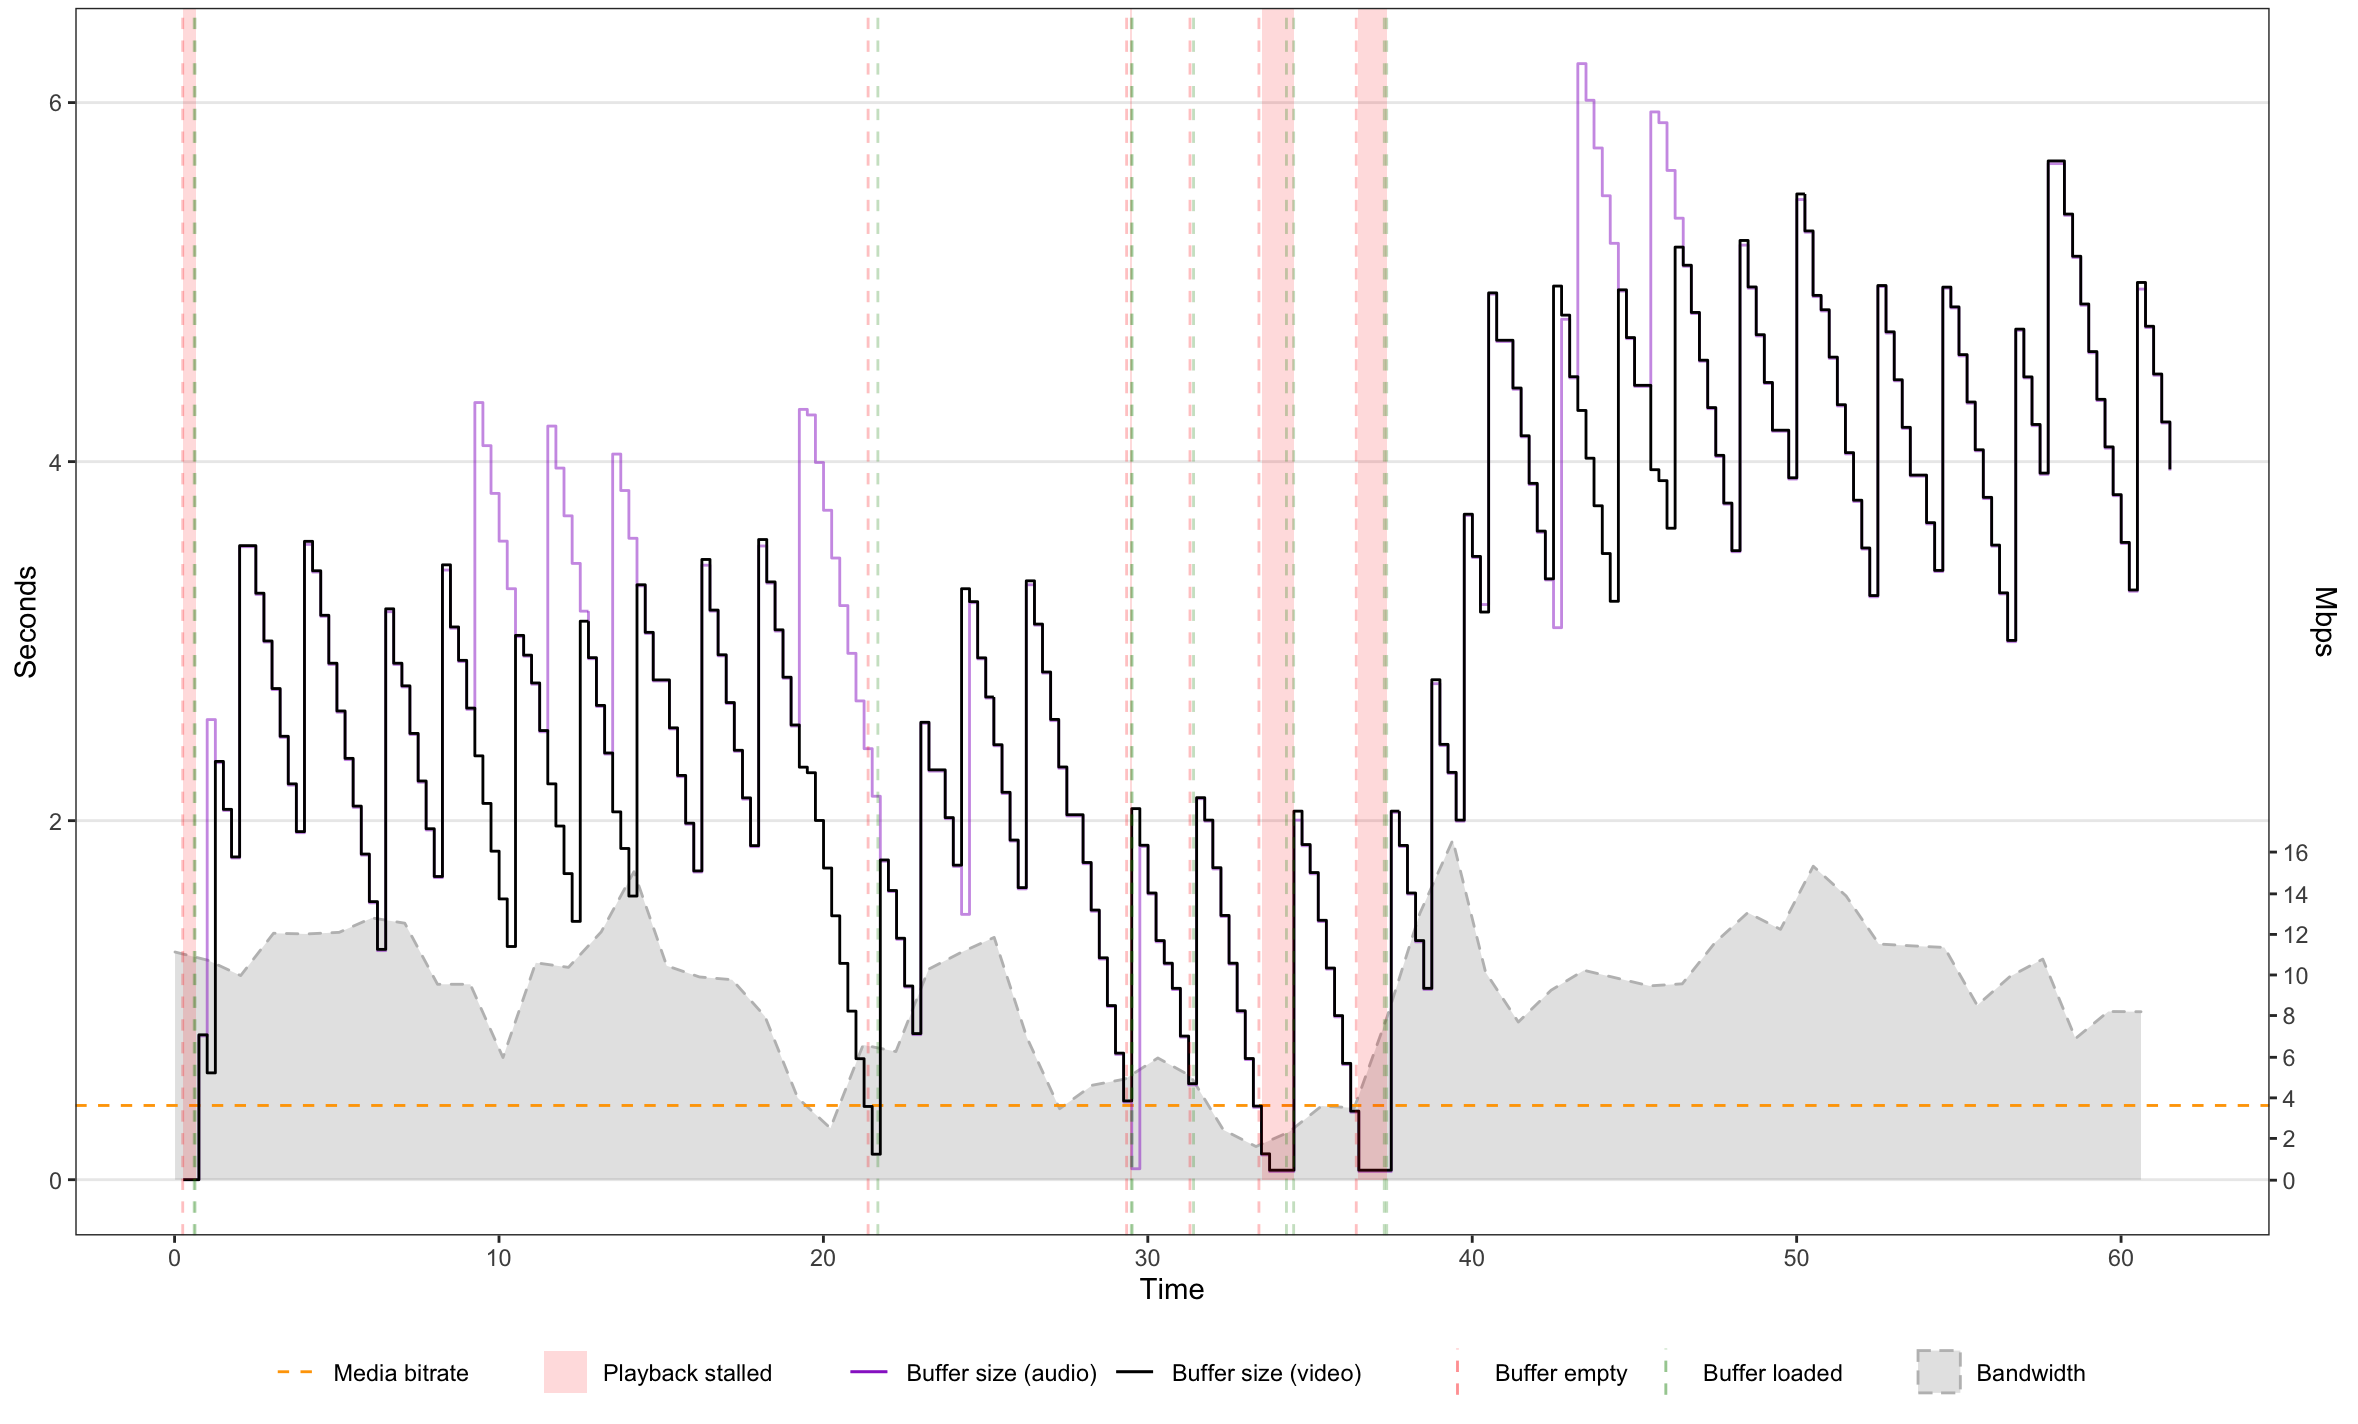
\includegraphics[width=0.9\textwidth]{res/eval_nonabr_lte_h3.png}
    \caption{Caption}
    \label{fig:eval_nonabr_lte_h3}
\end{figure}

What we can observe from the plot is that for the first 30 seconds the bandwidth is generally above the bitrate of the media, and therefore the buffer can be filled properly most of the time. One thing we can already observe is that the audio buffer is sometimes filled with more seconds of data than the video buffer. This happens because the video and audio tracks are unmuxed and can therefore be downloaded independently by the player/browser. Depending on the HTTP response scheduling, the audio segment might arrive before the video segment, or vice versa.

In the first half of the experiment, we can also notice a couple of cases where the player struggles to fill the video buffer in time. For example, just after second 20 the video buffer actually becomes empty for a very short period of time. As we will see later, in practice this kind of event does not necessarily produce a playback stall due to the way Chromium handles empty buffers.

At about second 30, the bandwidth starts to become very limited and goes below 3.5 Mbps for a few seconds. The video and audio buffers quickly deplete, empty buffer events are emitted, and playback stalls. This happens twice, as can be seen by the two red areas.

When the network bandwidth grows again, the buffers are filled. One thing to note is that the buffer length now contains about one segment more on average (closer to 3 seconds than to 2). This is because the delay introduced by the stall caused the playback to get behind with respect to the edge of the playlist, and therefore there is now an additional segment that can be loaded in advance.

The effect of this behavior can be seen better in the live latency plot, shown in Figure \ref{fig:eval_nonabr_lte_h3_latency}. In correspondence of the playback stalls, the live latency grows from about 4.5 to 5.5 seconds, and then to 6.5 seconds (in total, a 2-second segment more).

\begin{figure}[h]
    \centering
    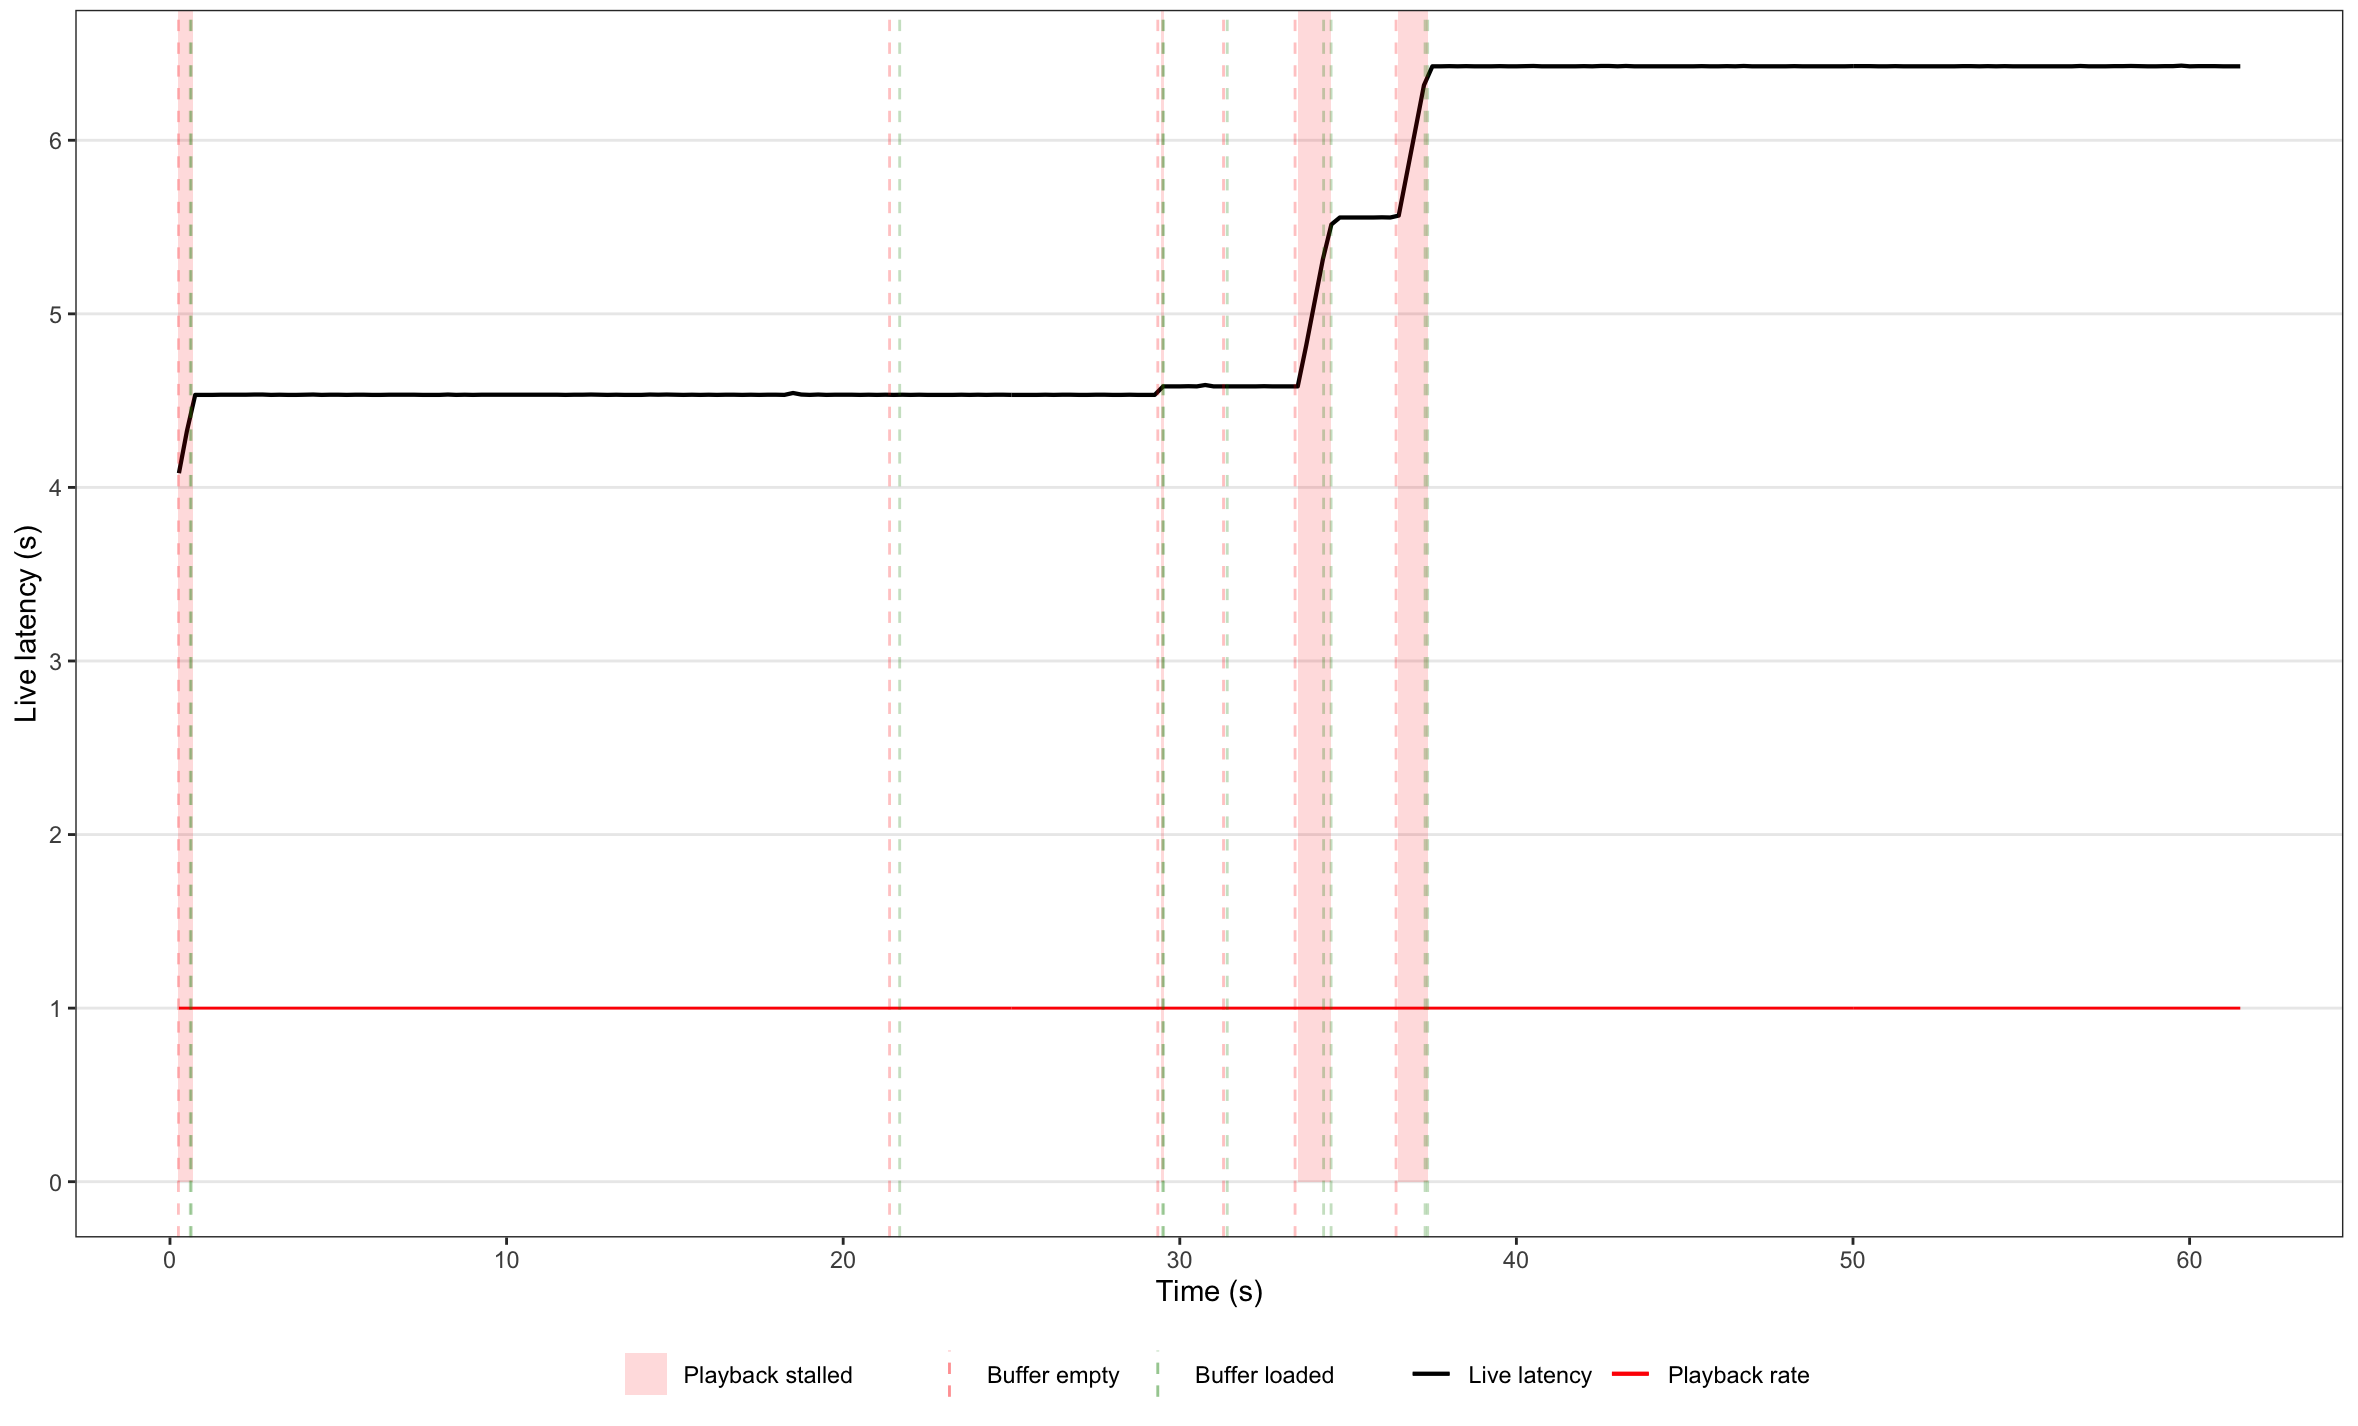
\includegraphics[width=0.9\textwidth]{res/eval_nonabr_lte_h3_latency.png}
    \caption{Caption}
    \label{fig:eval_nonabr_lte_h3_latency}
\end{figure}

Finally, if we observe the waterfall diagram (Figure \ref{fig:eval_nonabr_lte_h3_waterfall}, an interesting and perhaps unexpected behavior can be observed. Intuitively, we would expect request for audio segments to always take less time than video segments. In fact, while a single video segment can be as large as 1 MB, the audio segment is usually about 30 KB in size. This is usually between 10 and 30 times smaller than video. However, the waterfall shows that, while sometimes the loading of the audio segment takes very little time, the loading of the audio segments takes as long as the video.

\begin{figure}[h]
    \centering
    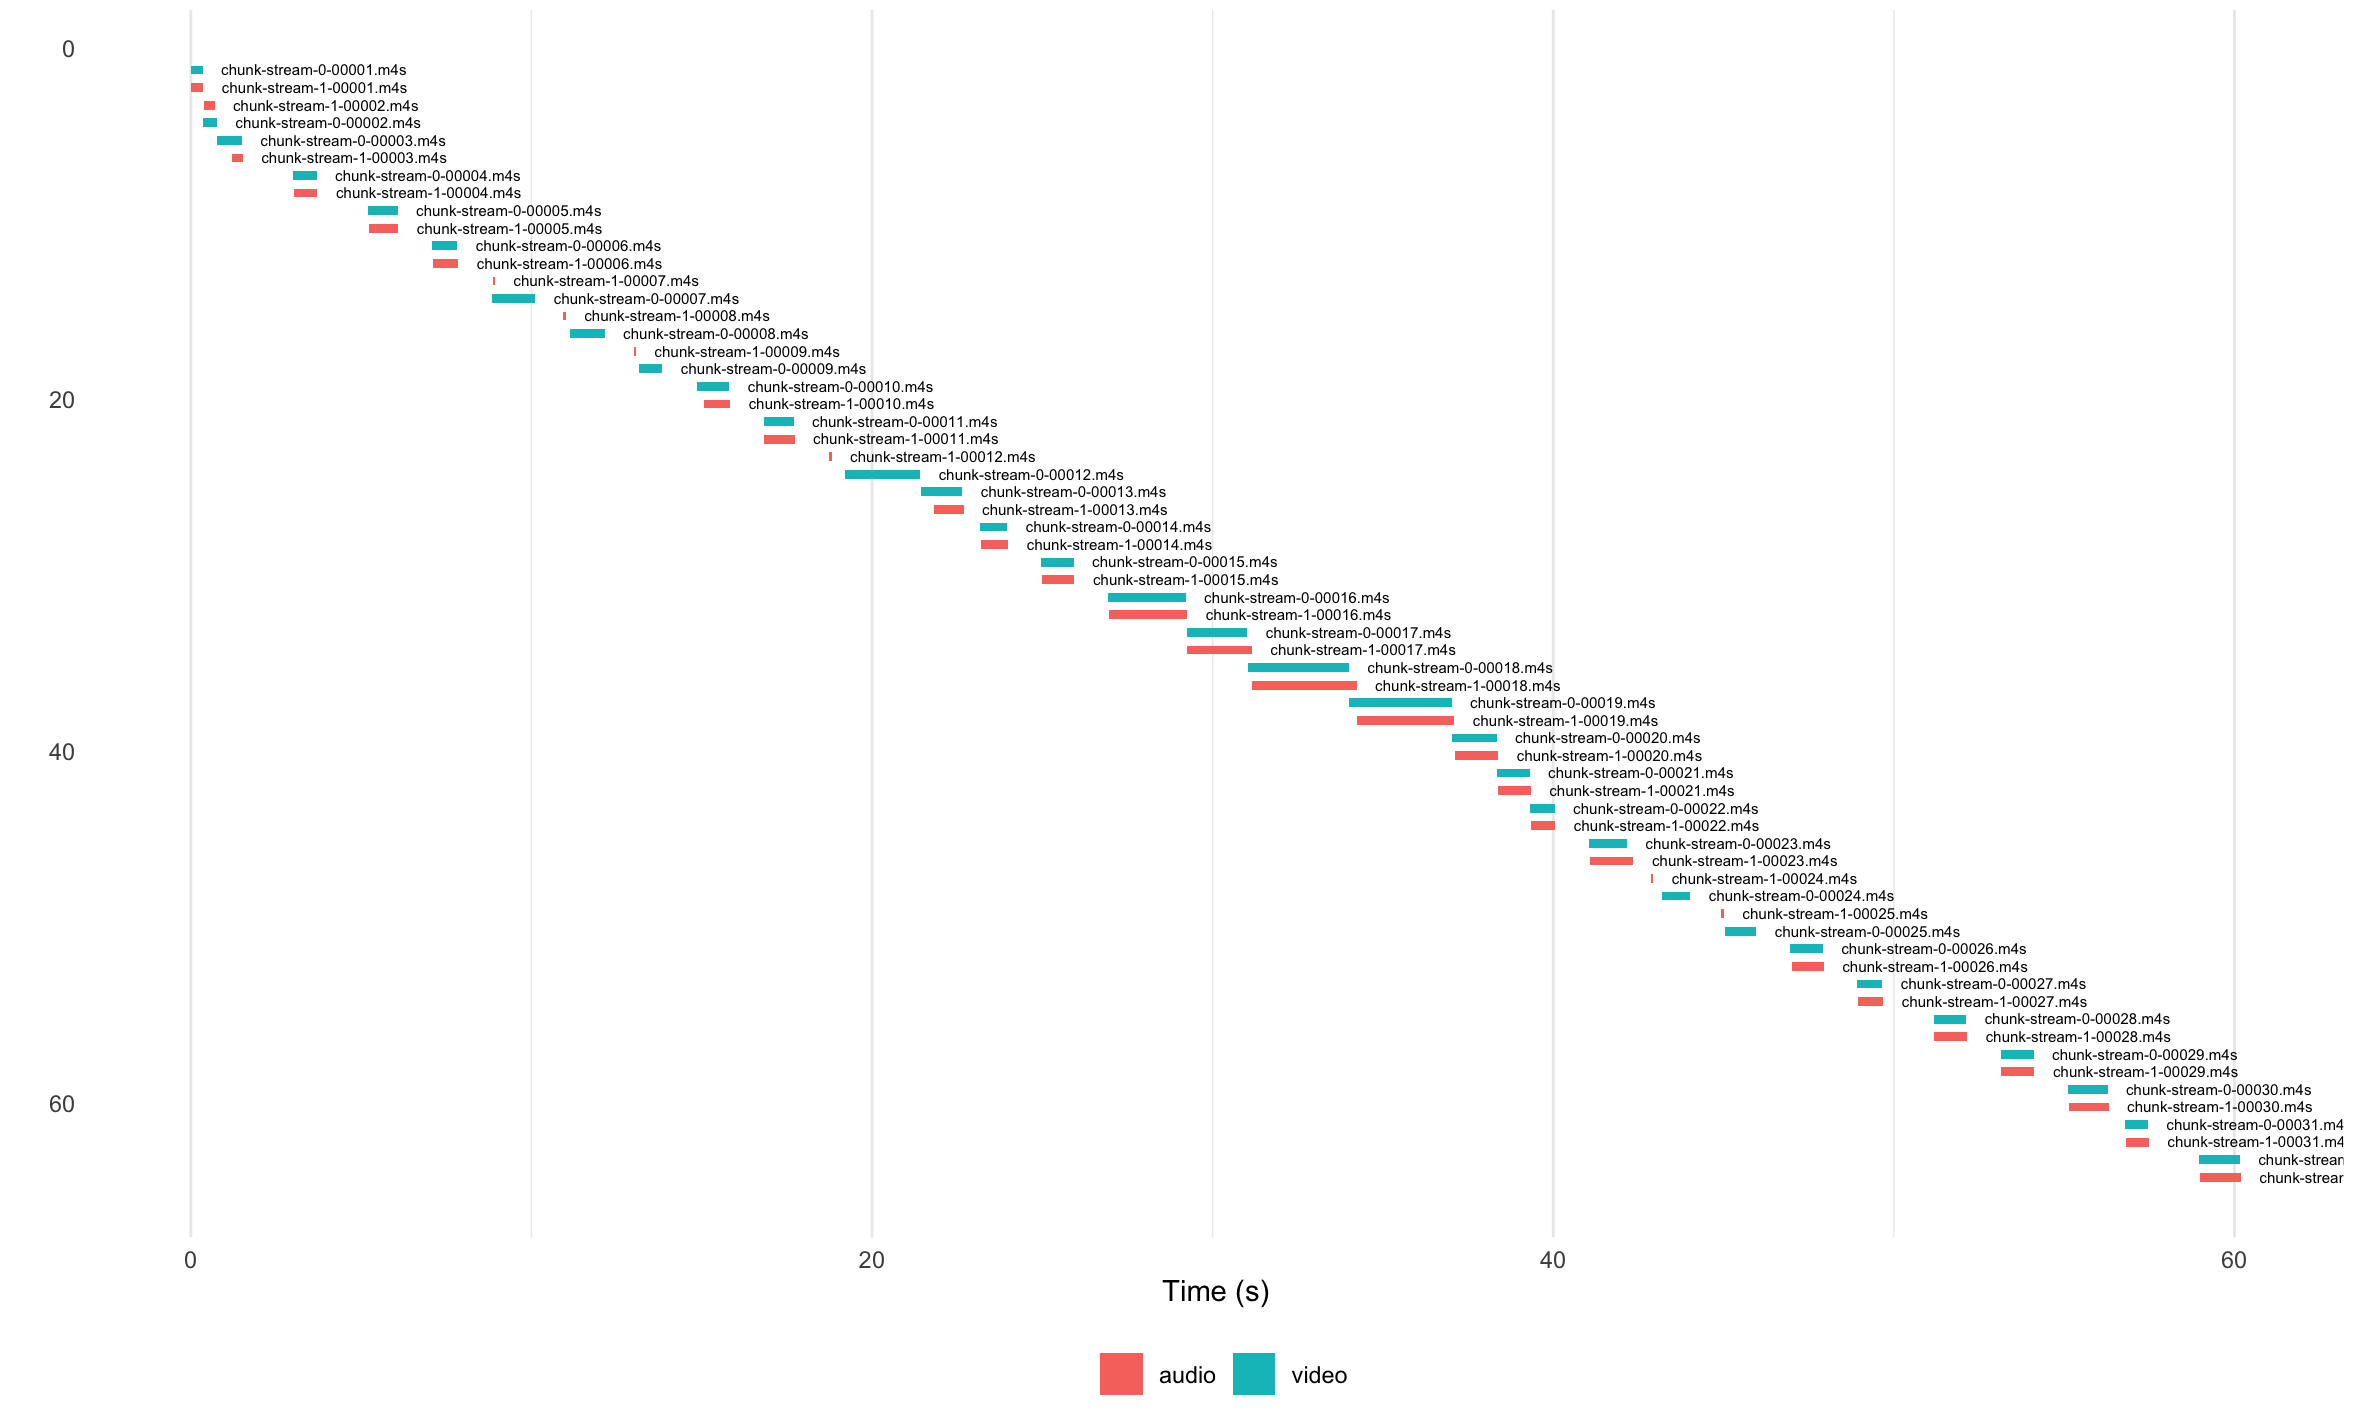
\includegraphics[width=0.9\textwidth]{res/eval_nonabr_lte_h3_waterfall.png}
    \caption{Caption}
    \label{fig:eval_nonabr_lte_h3_waterfall}
\end{figure}

This behavior hints at a suboptimal scheduling strategy of HTTP requests over the QUIC connection, so we decided to investigate this. We used the \textbf{NetLog dump} feature of Chromium (Section \ref{sec:bg/http3/tools}) to generate an export of network traffic, which also contains detailed information about QUIC connections and streams. We then analyzed the dump file with \textbf{qvis}.

One of the visualization tools provided by \textbf{qvis} is the multiplexing view, where the multiplexing of the streams at the QUIC level is represented both as a flow/timeline and as a waterfall (Figure \ref{fig:eval_noabr_qvis1}). The flow representation shows the sequence of QUIC packets that the client received. Each packet is colored with a different color depending on the stream to which it belongs. The waterfall view shows the same data as a waterfall chart, where each stream has its own row, and the horizontal segments represent the time intervals in which the stream was actively being transferred.

In our case, what we can clearly see in the multiplexing diagrams, especially in the waterfall, is that the streams are transmitted almost sequentially. In fact, there is almost no preemption, and most streams get to use the entire channel for transmission until all data is received.

\begin{figure}[h]
    \centering
    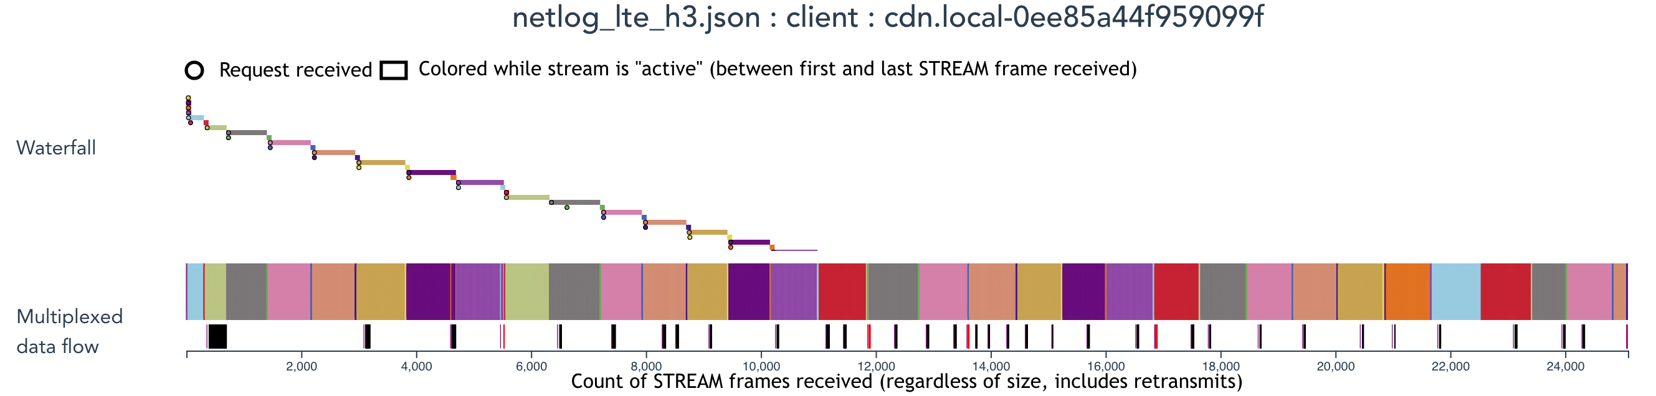
\includegraphics[width=0.9\textwidth]{res/eval_nonabr_qvis1.png}
    \caption{Caption}
    \label{fig:eval_noabr_qvis1}
\end{figure}

However, an interesting fact to observe is that the data flow is not entirely sequential. As Figure \ref{fig:eval_noabr_qvis2} shows, there is a recurring pattern of streams/requests that start and are immediately suspended to give bandwidth to another stream on the QUIC connection.

This behavior explains what we were seeing in the segments requests waterfall in Figure \ref{fig:eval_nonabr_lte_h3_waterfall}. Requests for audio and video segments often start at the same time; however, the transfer of the audio segment is almost immediately preempted to give priority to the video segment. The audio segment transfer is then completed after the video segment is completely downloaded.

This behavior is not ideal, because the audio segment is always much smaller than the video segment and thus could benefit from being transmitted earlier, as we will see in the next section. The next section will also compare how this same setup performs with HTTP/2 and HTTP/1.1, showing that the scheduling scheme that was observed seems to be specific to HTTP/3, or at least to the HTTP/3 implementation that we are relying on.

The takeaway result of this analysis is that we cannot rely on HTTP/3 implementations to always know the best strategy for request prioritization. Instead, it is also the client/browser's responsibility to implement optimizations so that the prioritization strategy is meaningful.

The prioritization strategy could derive from browser heuristics that are applied globally for all websites, as we mentioned in Section \ref{sec:bg/http2}, but it could also be explicitly requested by developers.

\begin{figure}[h]
    \centering
    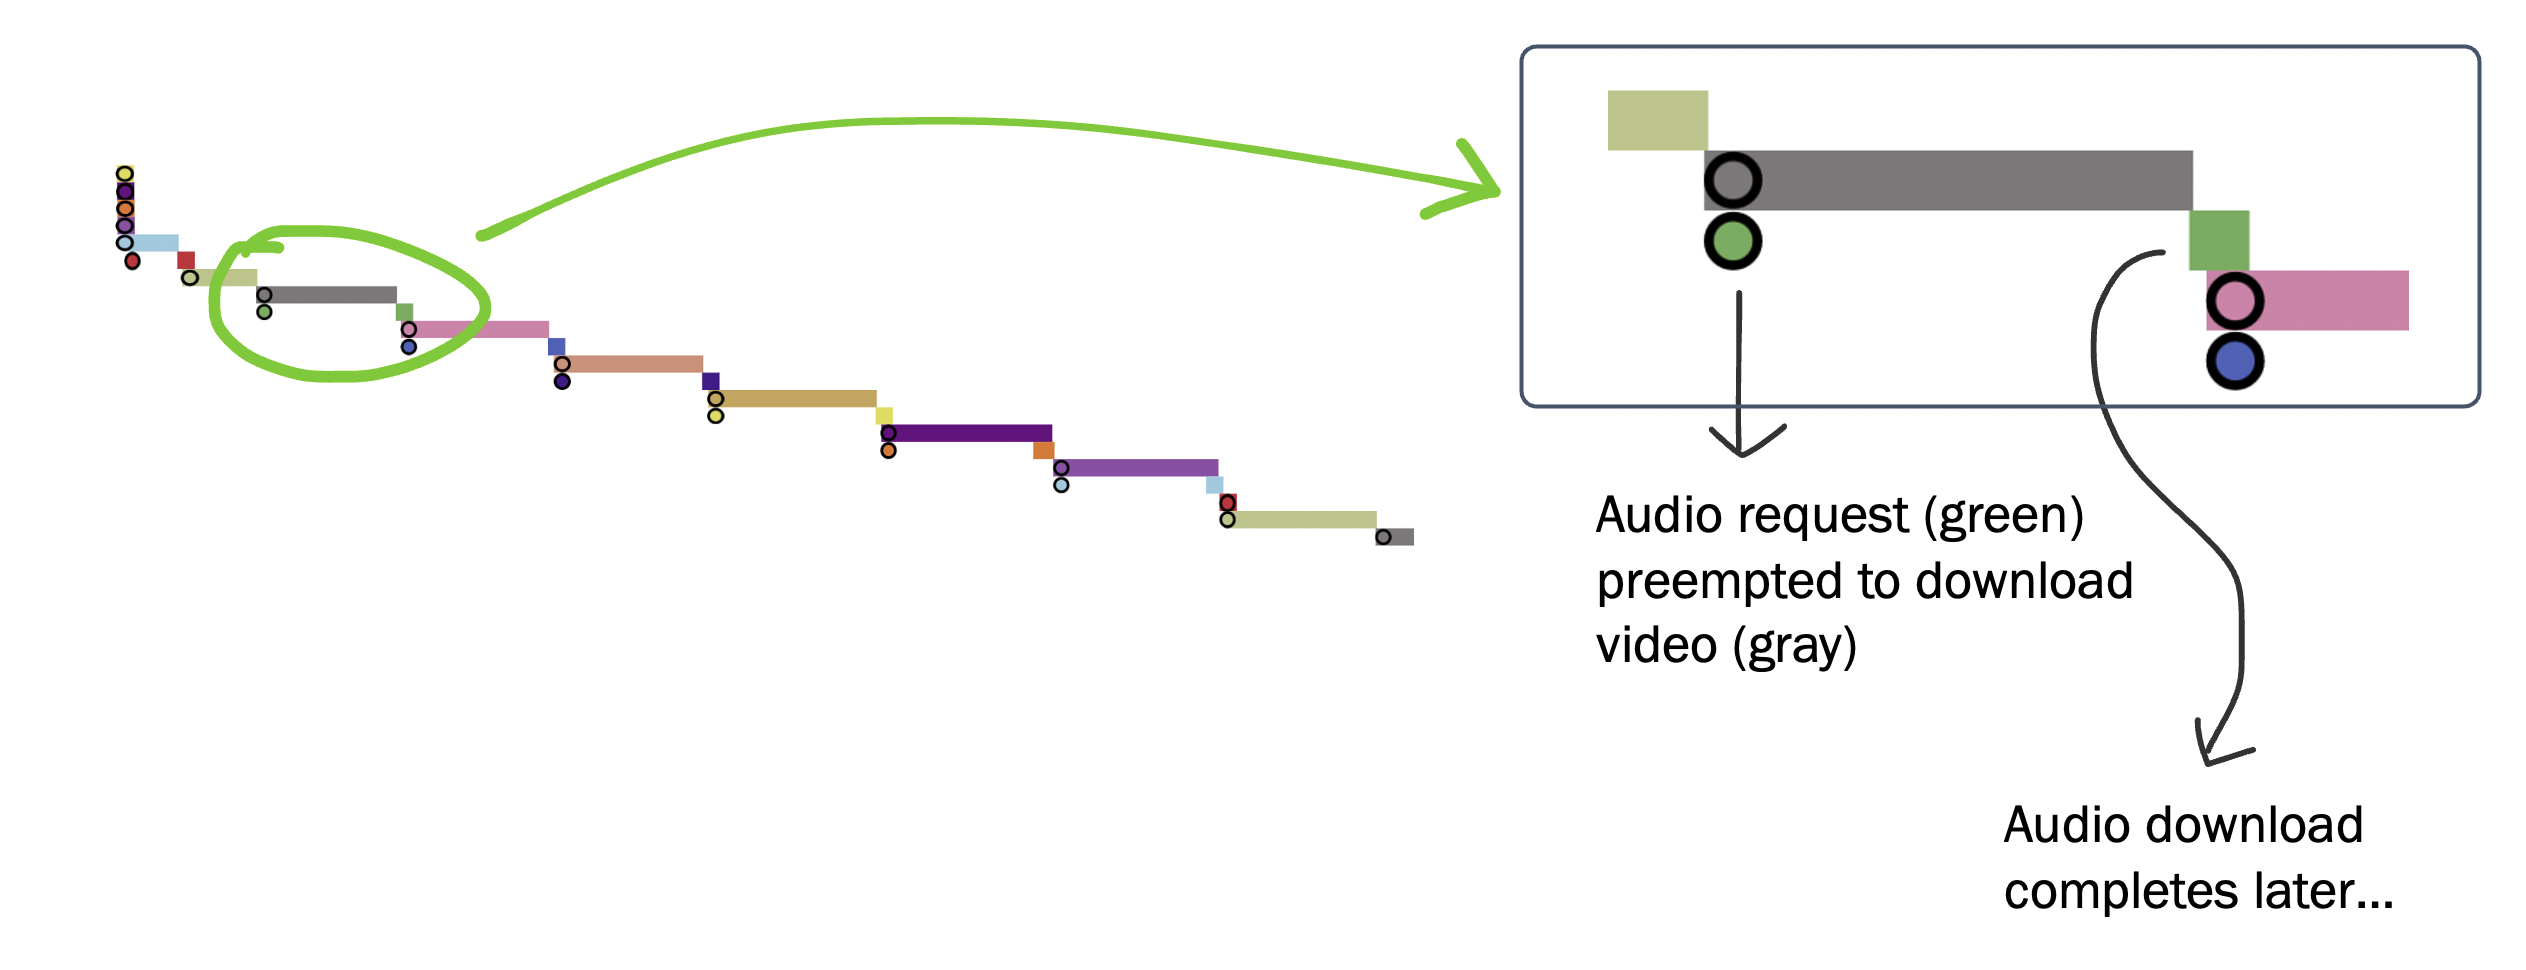
\includegraphics[width=0.9\textwidth]{res/eval_nonabr_qvis2.png}
    \caption{Caption}
    \label{fig:eval_noabr_qvis2}
\end{figure}

\subsubsection{Comparison across HTTP versions}
\label{sec:eval/non-abr/http-versions}

As we have seen, the emulation over HTTP/3 shows that priorities are not consistent, even in the same run. We will now see how HTTP/2 and HTTP/1.1 behave and compare the results.

Let us start from HTTP/2. Figure \ref{fig:eval_nonabr_lte_h2_buffer} shows the buffer health plot for an experiment execution based on HTTP/2. The rest of the settings remained the same. As we can easily see, the behavior is quite different from HTTP/3. First, the audio buffer is always larger than the video. This means that the audio segments are consistently loaded before the video buffer. The waterfall in Figure \ref{fig:eval_nonabr_lte_h2_waterfall} confirms that this is because the audio segments are loaded much faster, as we would expect, and the loading of the video segments does not delay the audio. This behavior probably derives from a different prioritization strategy, implemented by the browser or driven by the HTTP/2 server implementation.

The other thing that we can observe is that there are no playback stalls, apart from the initial loading, even if the video buffer is almost empty for several seconds in the middle of the emulation. This behavior derives from the fact that the browser is capable of playing the audio data even if the video is not available, for up to 3 seconds. This particular underflow behavior is specific to Chromium and is officially documented. Obviously, it can only work when audio and video data is appended to the MSE \texttt{SourceBuffer} independently; therefore, in practice it can only happen when using unmuxed video and audio tracks, as in our case.

Although Chromium's underflow behavior might not be the expected experience when streaming on-demand content, since it has the effect of freezing the video for a few seconds, it is instead particularly suitable for live streaming. In fact, in this way short time intervals where video data is not available do not cause a stall, and, therefore, do not increase the latency of the live streams. While the video is frozen due to a slow loading segment, the audio will continue to play.

\begin{figure}[h]
	\centering
	
	\begin{subfigure}[t]{0.45\textwidth}
		\centering
		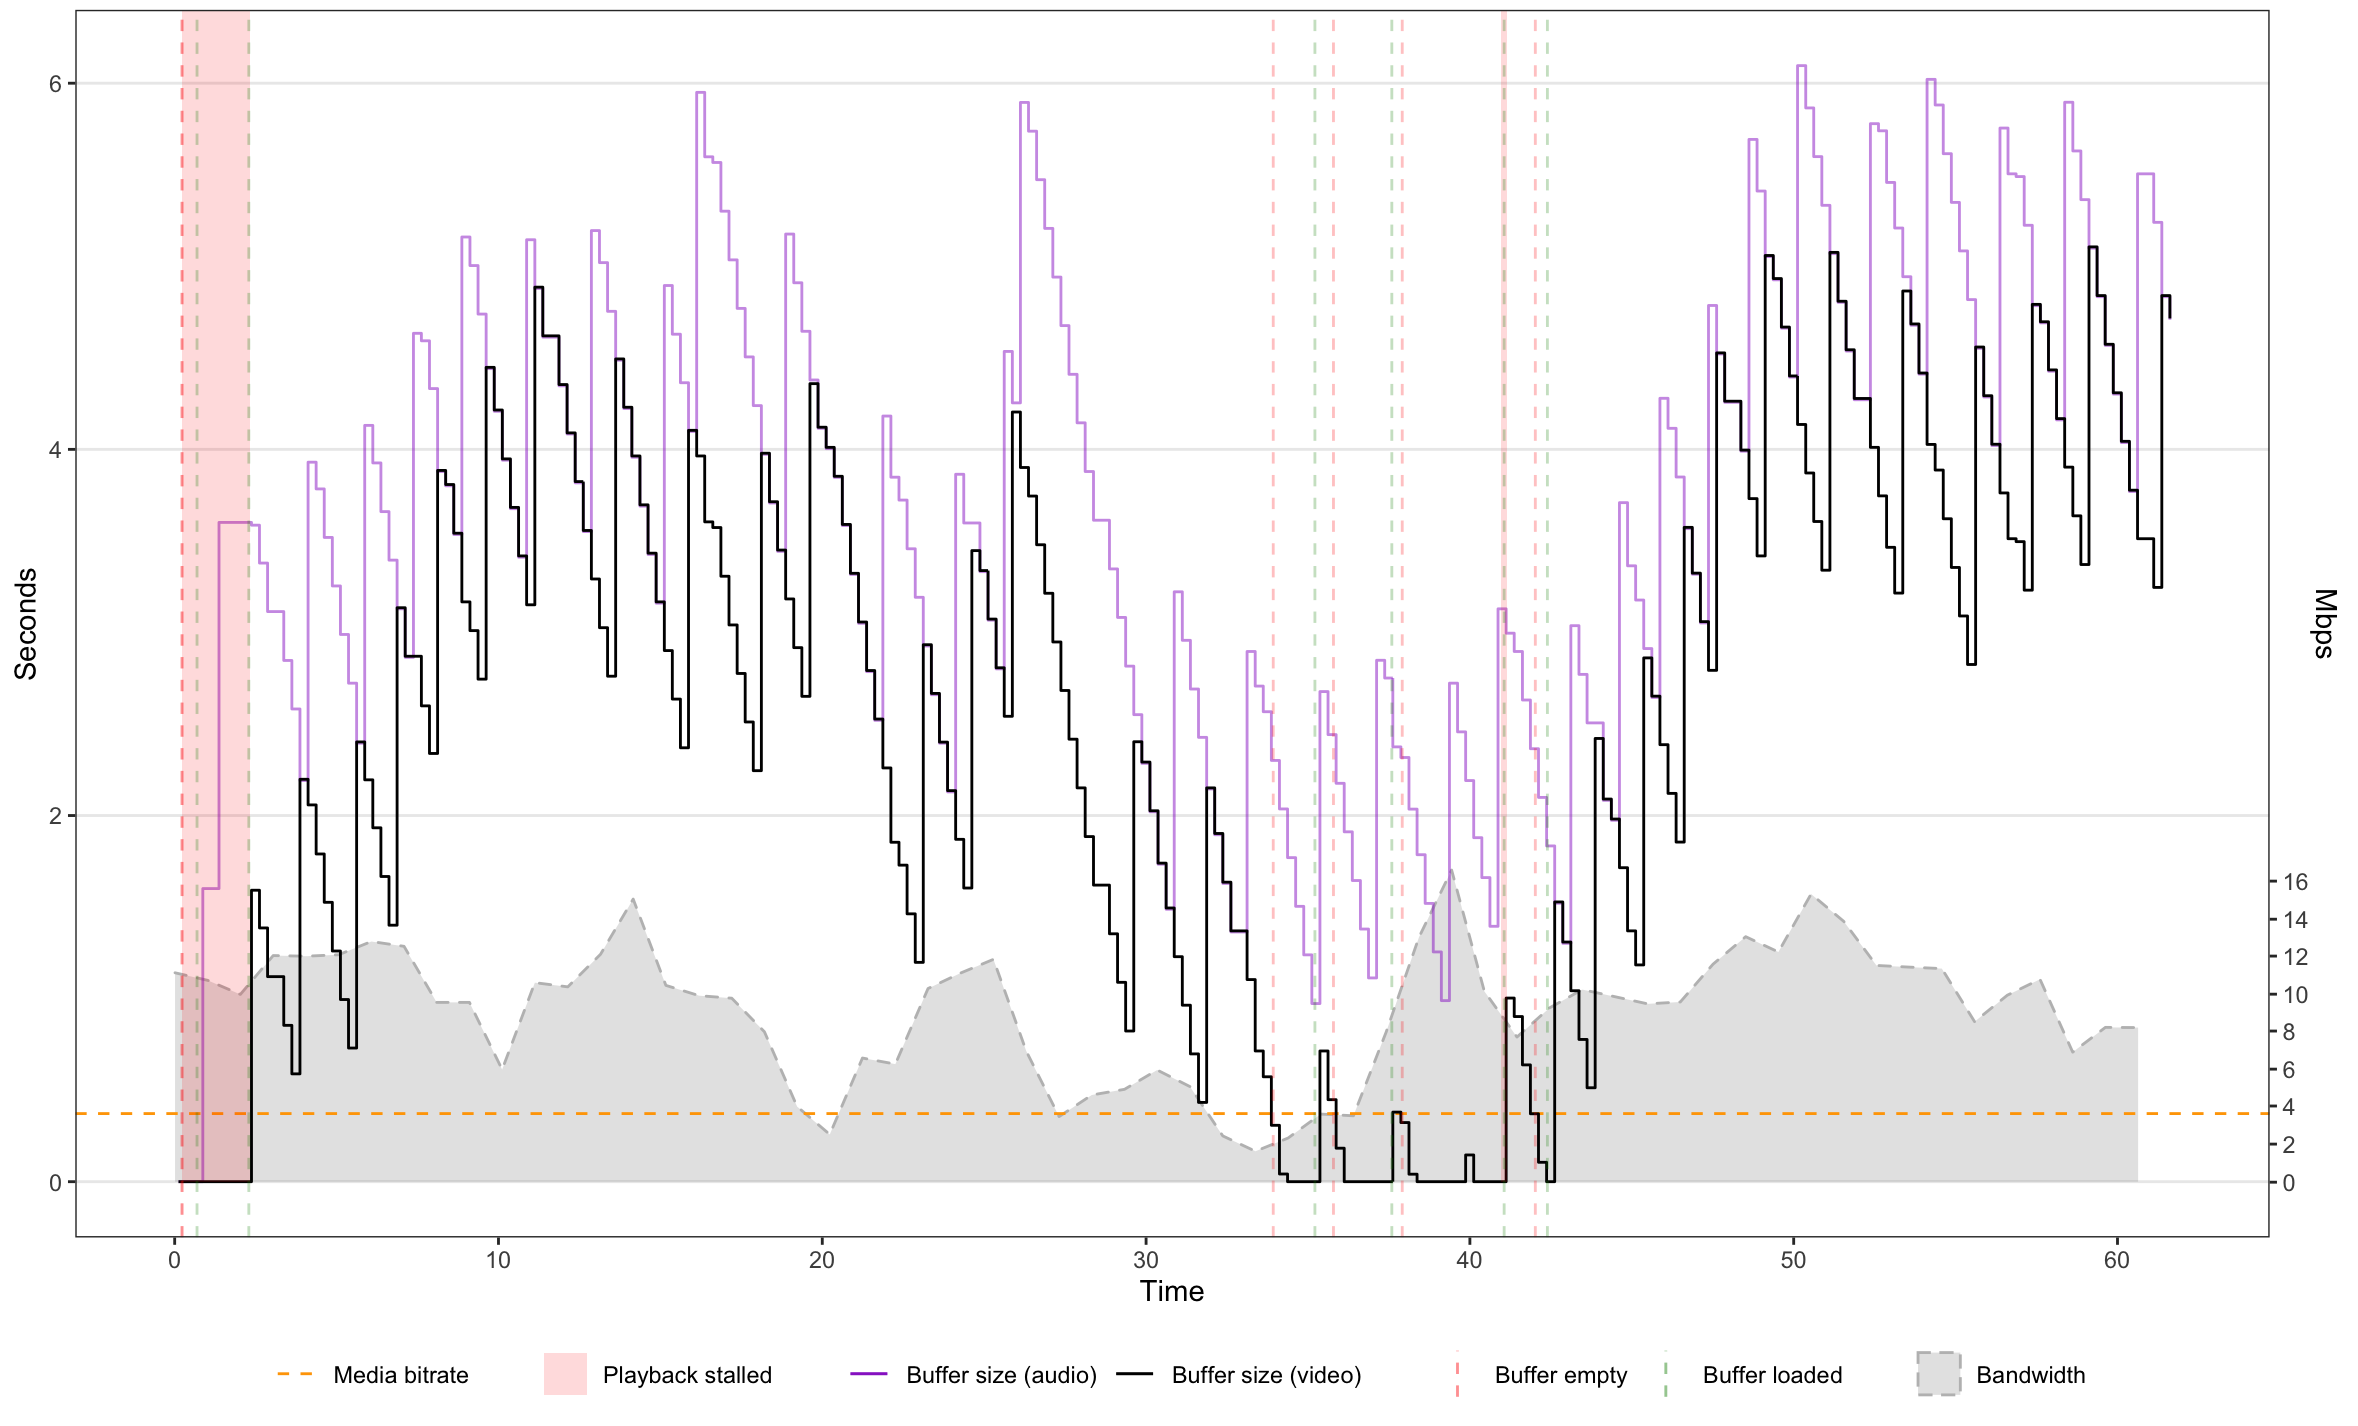
\includegraphics[width=\textwidth]{res/eval_nonabr_lte_h2.png}
		\caption{Caption}
		\label{fig:eval_nonabr_lte_h2_buffer}
	\end{subfigure}%
	~ 
	\begin{subfigure}[t]{0.45\textwidth}
		\centering
		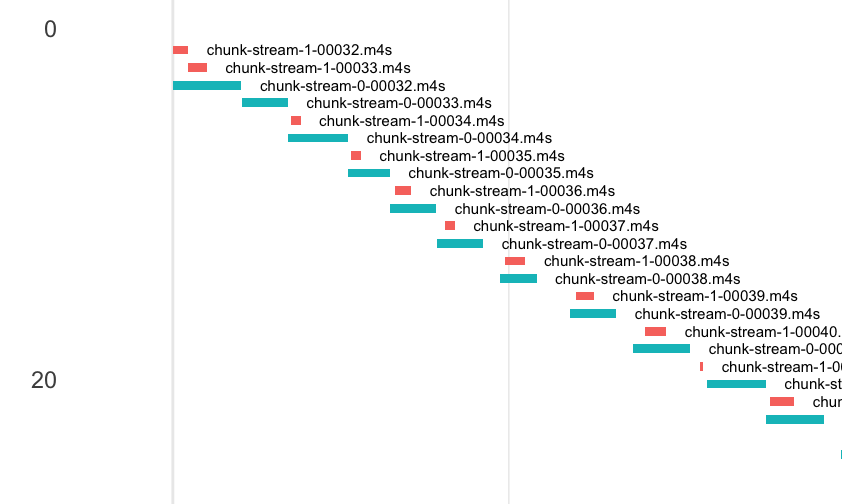
\includegraphics[width=\textwidth]{res/eval_nonabr_lte_h2_waterfall.png}
		\caption{Caption}
		\label{fig:eval_nonabr_lte_h2_waterfall}
	\end{subfigure}
	
	\caption{Caption}
	\label{fig:eval_nonabr_lte_h2}
\end{figure}

Moving on to HTTP/1.1, the behavior that we observed is somewhat similar to HTTP/2. As Figure \ref{fig:eval_nonabr_lte_h1_buffer} shows, the audio buffer is virtually always longer than the video buffer. One thing to note is that there is a playback stall at about 38 seconds, even if the audio buffer contains several seconds of data. This is due to the limitations of the underflow tolerance that we have seen earlier: Chromium only allows the video track to have missing data for about 3 seconds, after which the playback will stall. We will tackle this limitation in Section X.

The waterfall diagram for HTTP/1.1, shown in \ref{fig:eval_nonabr_lte_h1_waterfall}, is perhaps even more interesting. It shows that the download of the audio segments, represented in red, is consistently completed in a very short amount of time. Intuitively, the explanation for this phenomenon is that HTTP/1.1 can use multiple independent TCP connections, not performing multiplexing at all. In this way, requests can be distributed among the connections and benefit from a "dedicated" transmission channel.

\begin{figure}[h]
	\centering
	
	\begin{subfigure}[t]{0.45\textwidth}
		\centering
		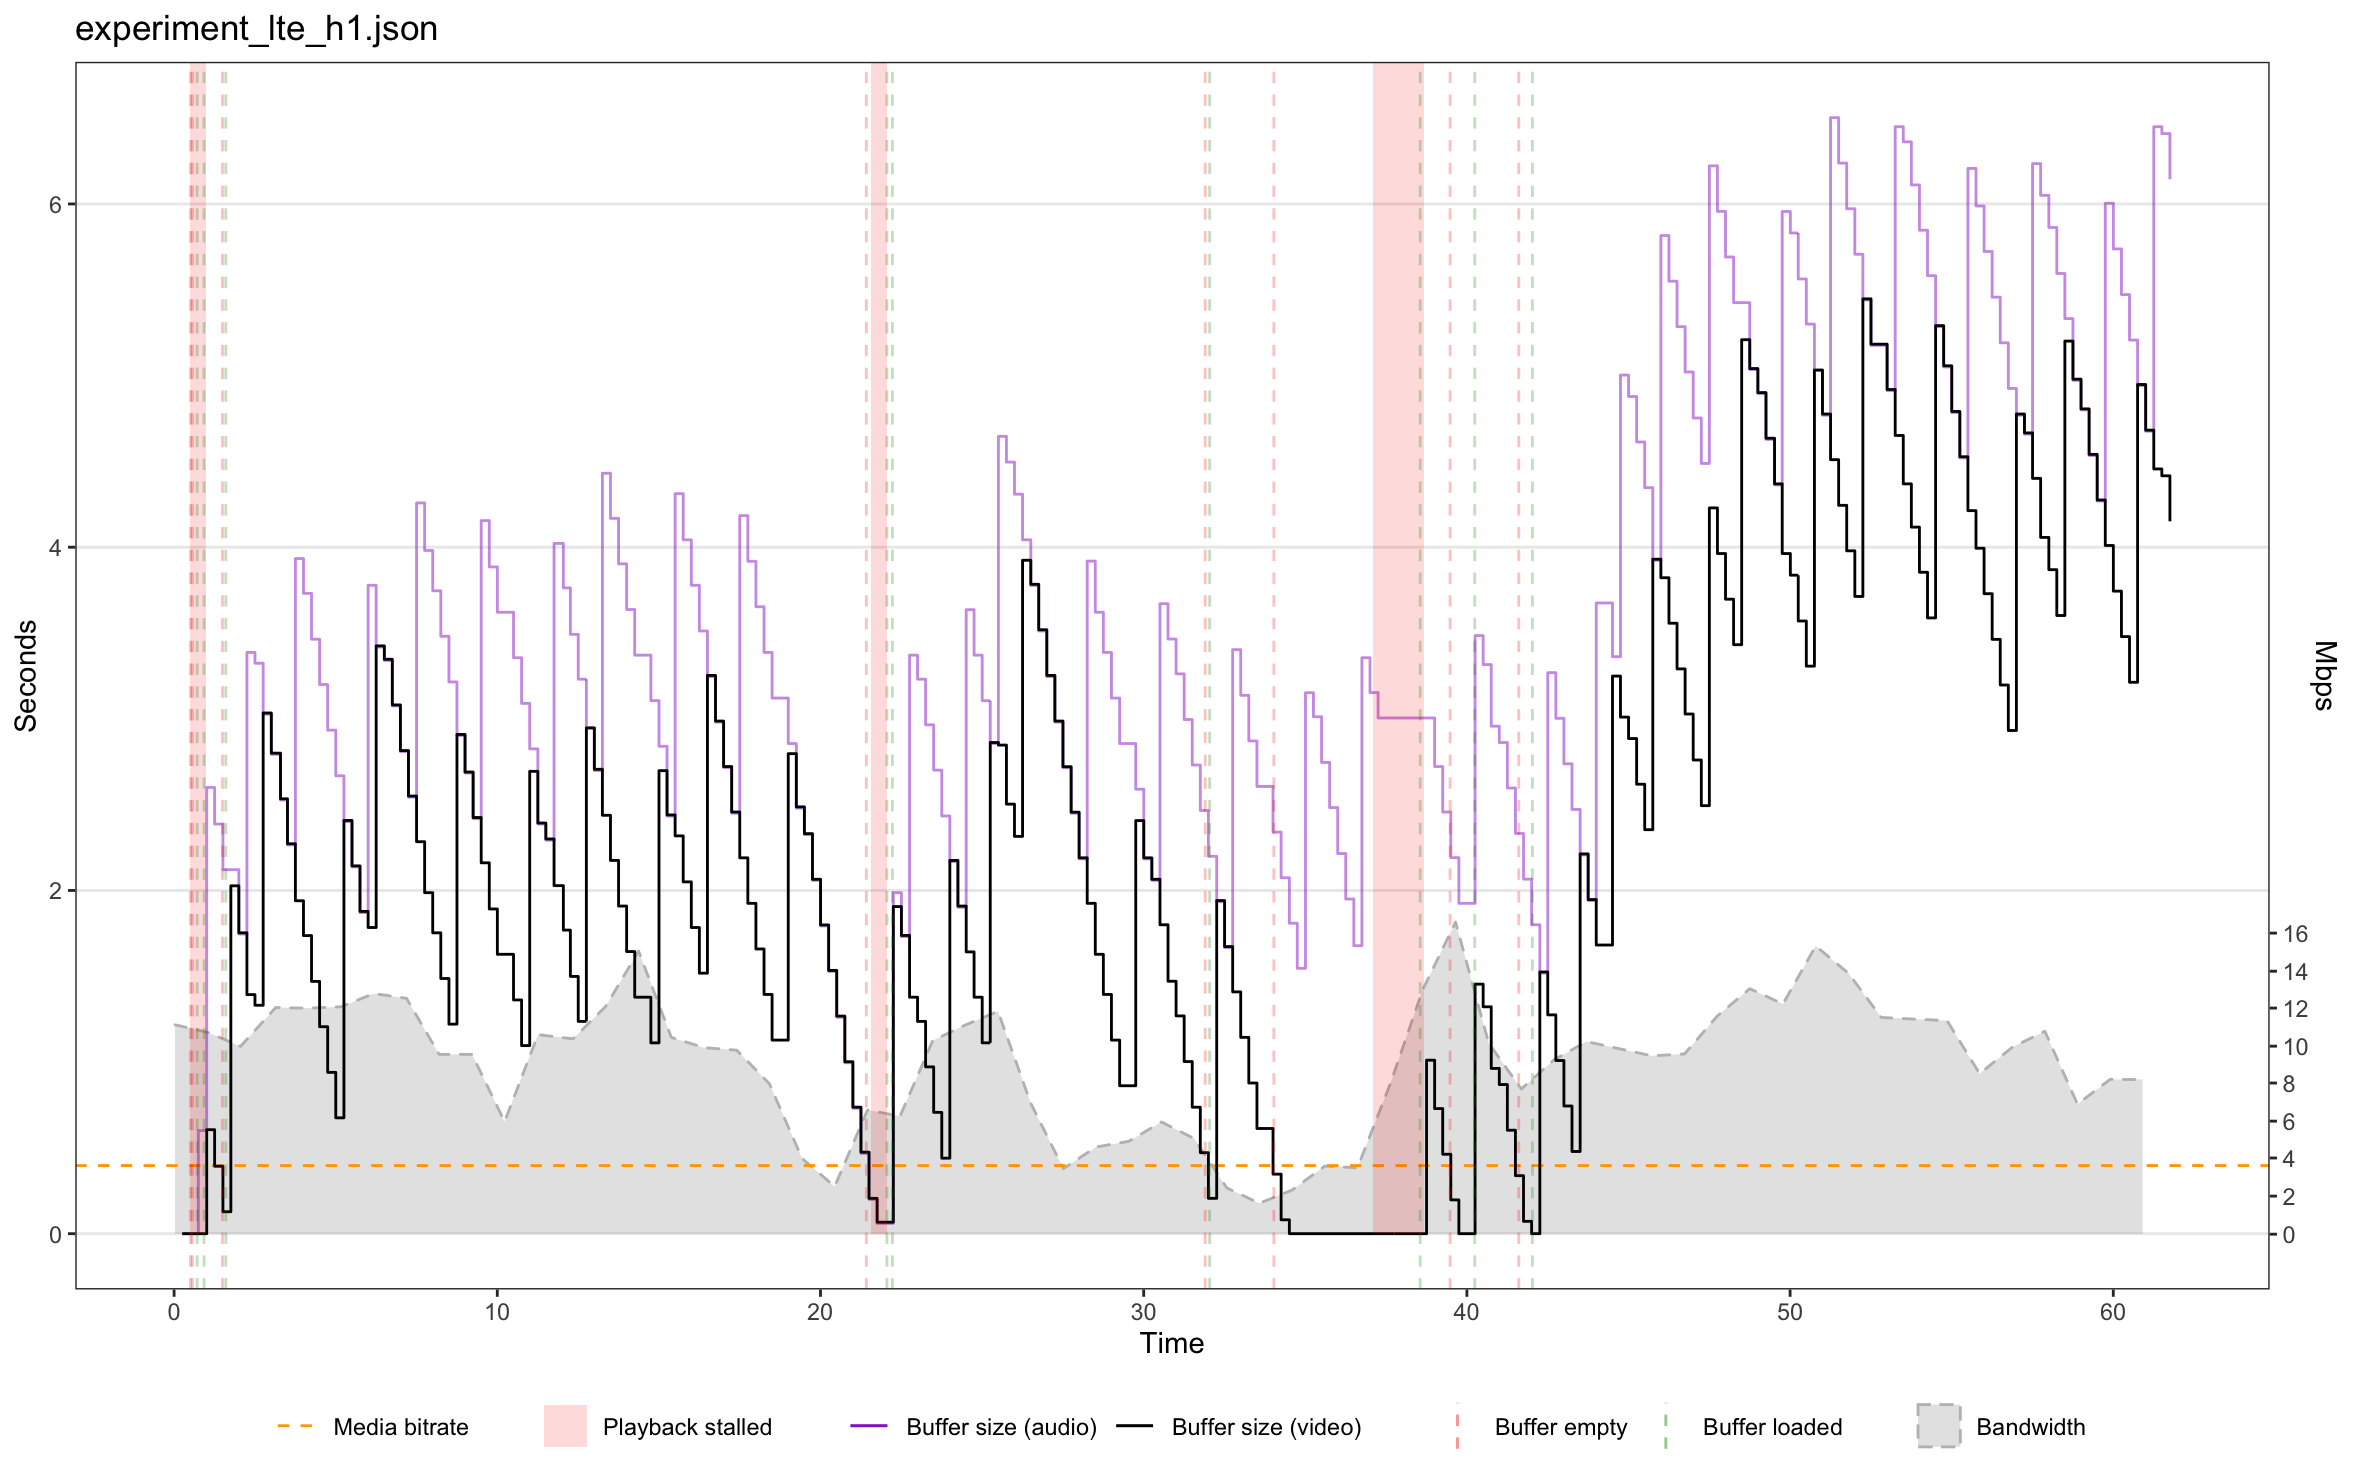
\includegraphics[width=\textwidth]{res/eval_nonabr_lte_h1.png}
		\caption{Caption}
		\label{fig:eval_nonabr_lte_h1_buffer}
	\end{subfigure}%
	~ 
	\begin{subfigure}[t]{0.45\textwidth}
		\centering
		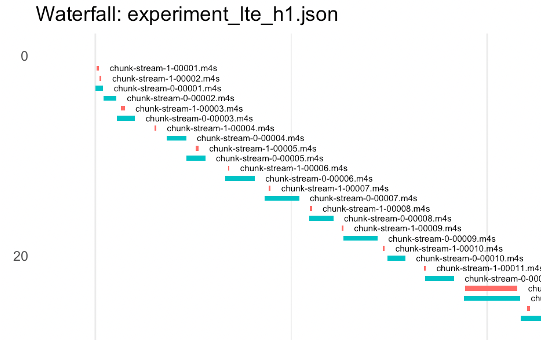
\includegraphics[width=\textwidth]{res/eval_nonabr_lte_h1_waterfall.png}
		\caption{Caption}
		\label{fig:eval_nonabr_lte_h1_waterfall}
	\end{subfigure}
	
	\caption{Caption}
	\label{fig:eval_nonabr_lte_h1}
\end{figure}

These results are surprising. We are seeing that HTTP/2 and HTTP/1.1 appear to offer better scheduling of requests. Incidentally, this also translates into a live streaming experience that has fewer "hard" stalls and where the latency does not increase.

\subsubsection{The need for adaptive bitrate streaming}
\label{sec:eval/non-abr/adaptive}

The experiments mentioned above were conducted with the \texttt{lte} network pattern, where the network bandwidth is most of the time higher than the media bitrate. In the \texttt{hspa+} pattern the situation is different: the bandwidth is just slightly above the media bitrate and often goes below it. This is pretty clear from Figure \ref{fig:eval_nonabr_hspa+_h3_buffer}, where there are many stalls in all situations where the bandwidth is not enough. The consequence is that the live latency increases during the playback stall periods, reaching 23 seconds as shown in \ref{fig:eval_nonabr_hspa+_h3_waterfall}.

\begin{figure}[h]
	\centering
	
	\begin{subfigure}[t]{0.45\textwidth}
		\centering
		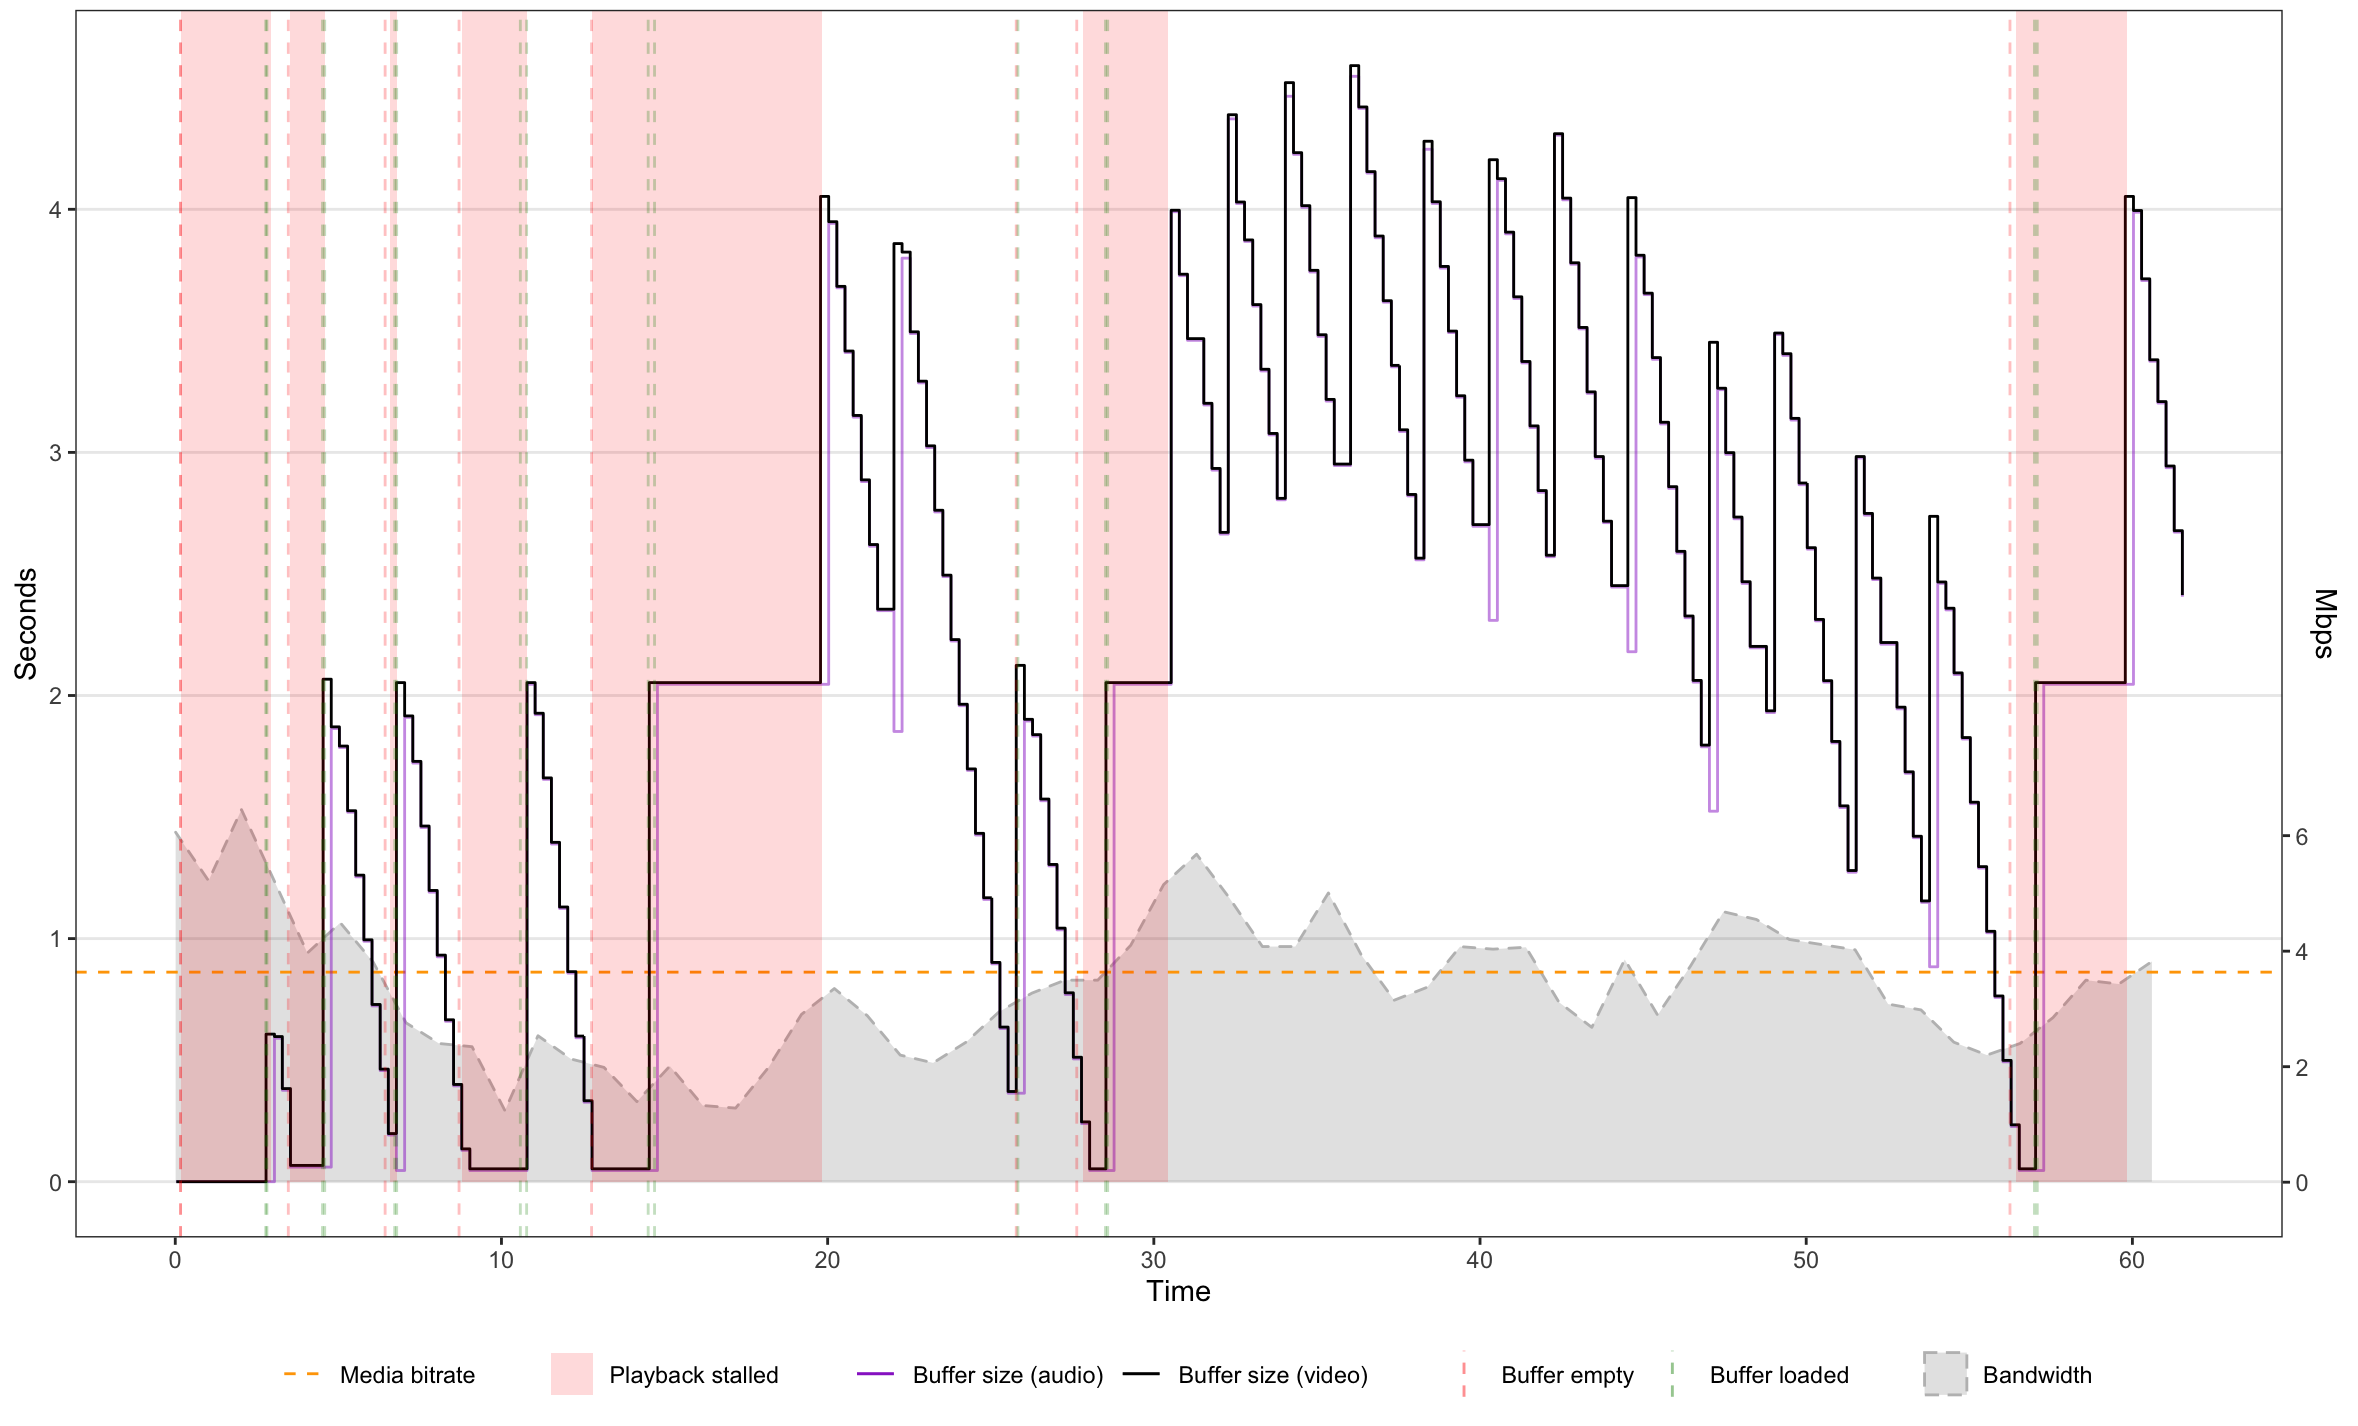
\includegraphics[width=\textwidth]{res/eval_nonabr_hspa+_h3.png}
		\caption{Caption}
		\label{fig:eval_nonabr_hspa+_h3_buffer}
	\end{subfigure}%
	~ 
	\begin{subfigure}[t]{0.45\textwidth}
		\centering
		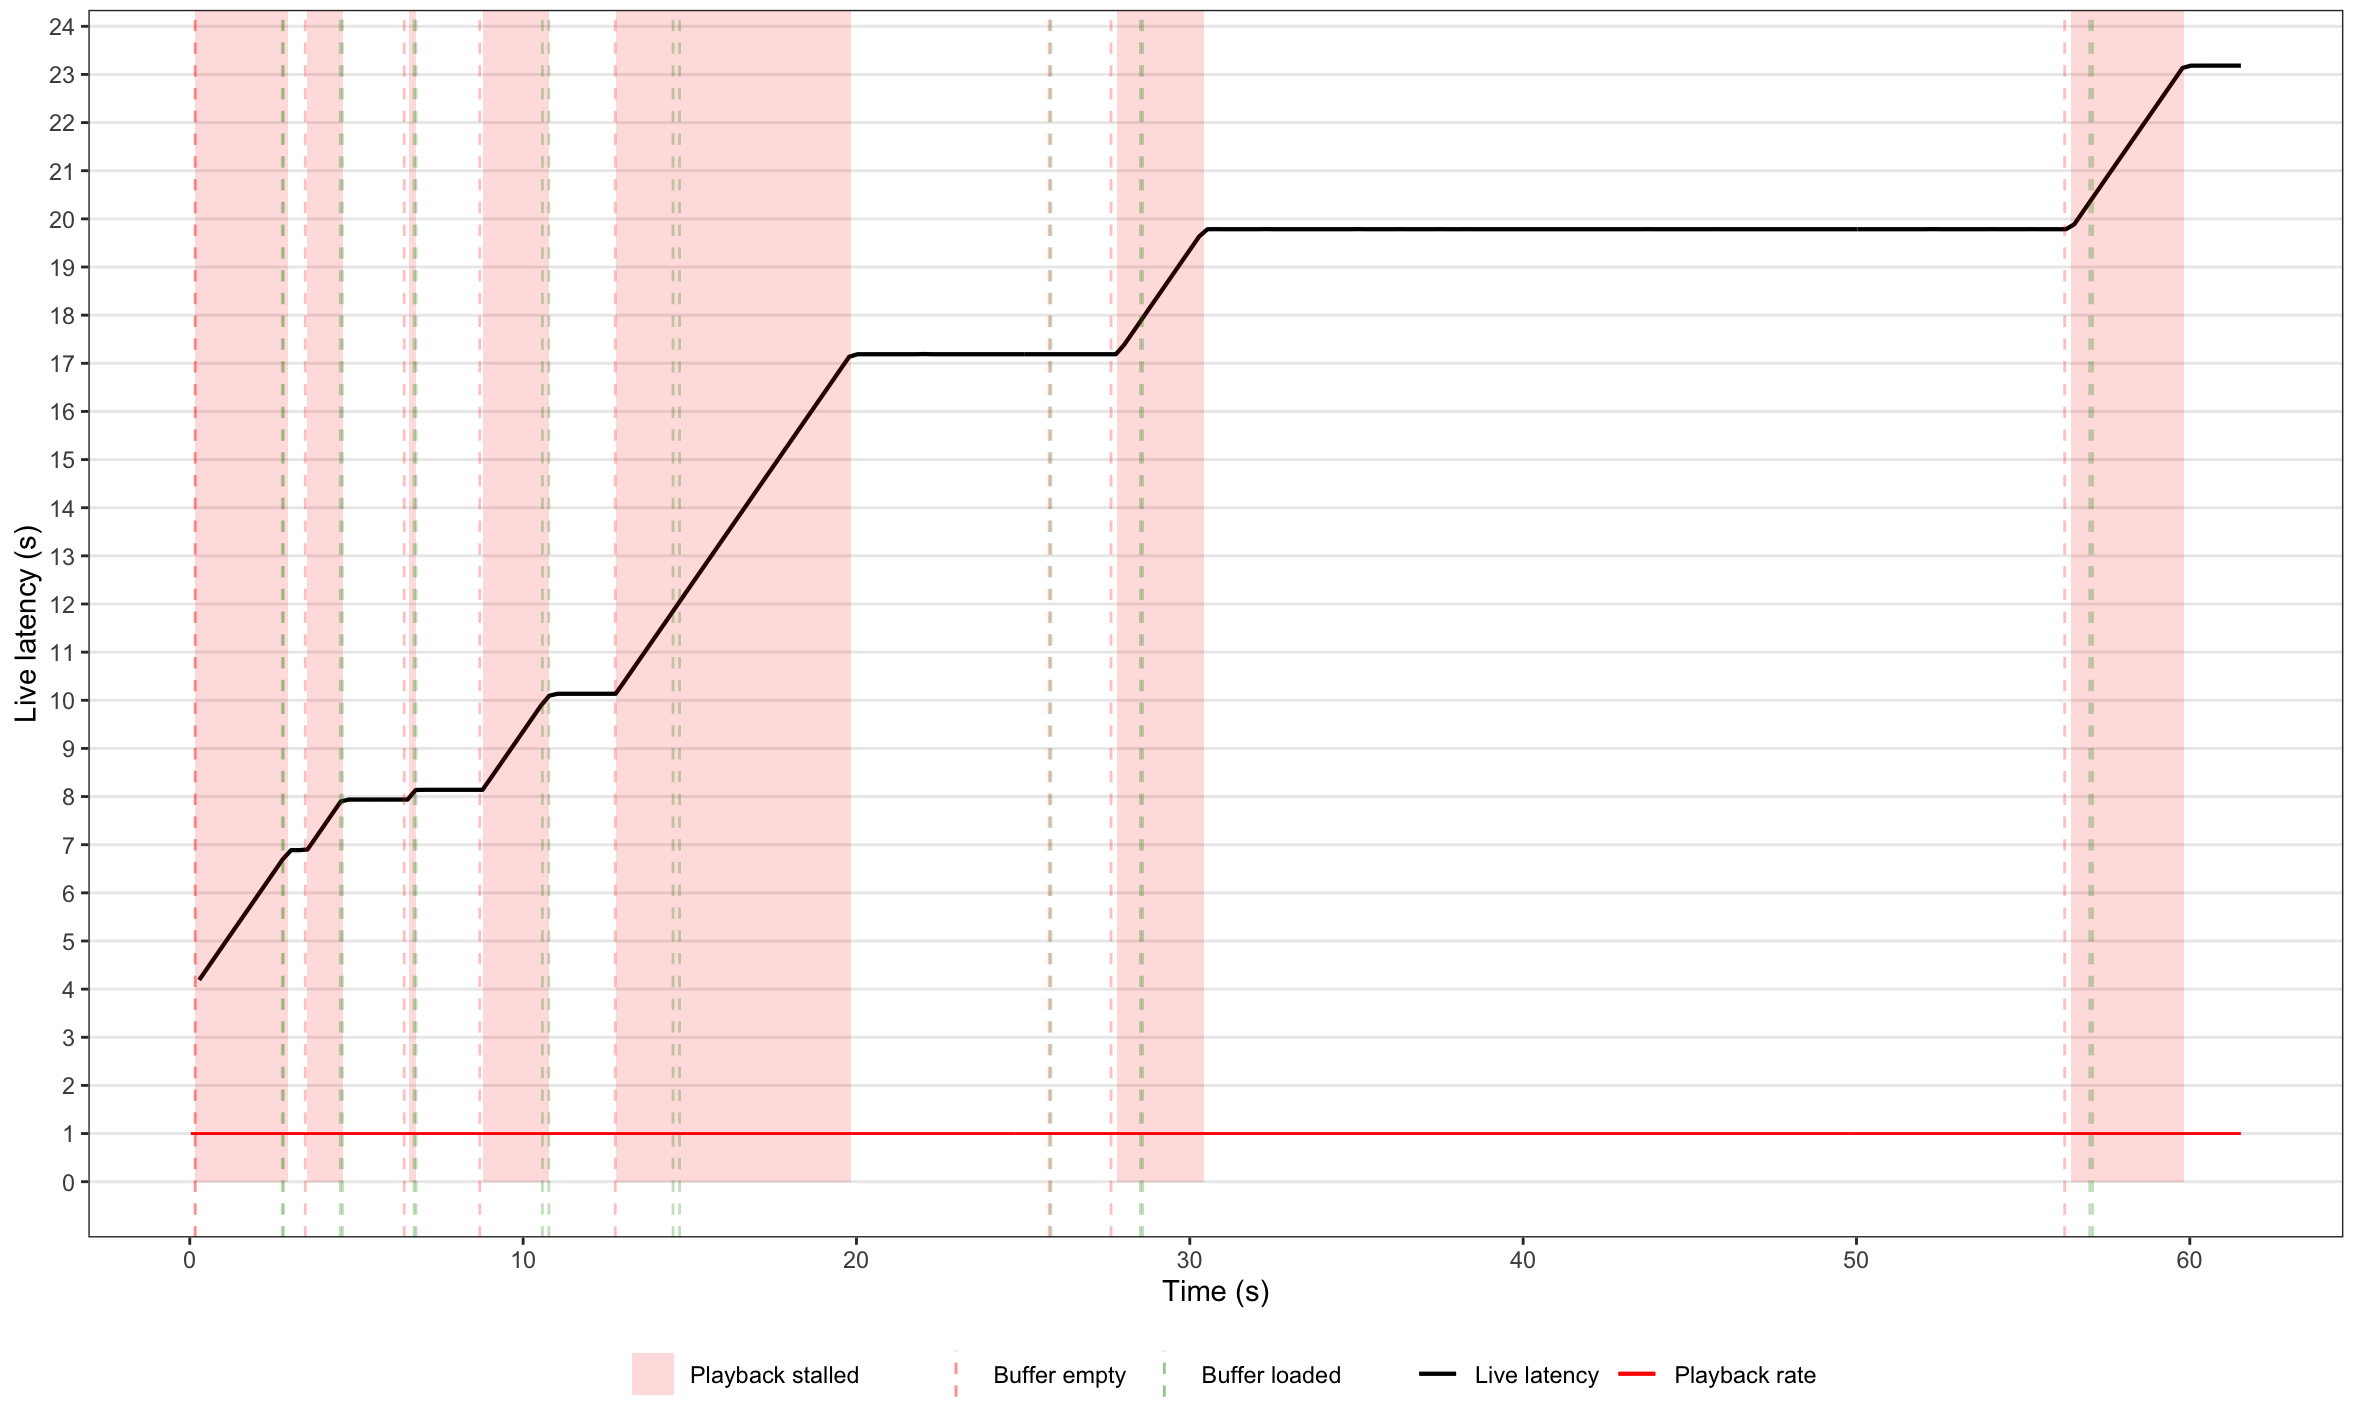
\includegraphics[width=\textwidth]{res/eval_nonabr_hspa+_h3_latency.png}
		\caption{Caption}
		\label{fig:eval_nonabr_hspa+_h3_waterfall}
	\end{subfigure}
	
	\caption{Caption}
	\label{fig:eval_nonabr_hspa+_h3}
\end{figure}

Adaptive bitrate streaming is needed for this reason: when the adaption algorithms estimates that there is not enough bandwidth to continue the playback at the current bitrate, it will make the decision to switch to a lower bitrate. In the next sections, we will see how the system performs when adaptive bitrate streaming is enabled.

\subsection{Experiments and results in an ABR setup}
\label{sec:eval/abr}

The testbed that we introduced in Section \ref{sec:eval/testbed} is already capable of running experiments on a live stream that is adaptive. In fact, if we do not specify the minimum bitrate in the experiment configuration the playback will be ABR. We tested this setup with both DASH.js and hls.js.

\subsubsection{Suboptimal behavior of the default DASH.js configuration with live}
\label{sec:eval/abr/dashjs}

An experiment we run involved using DASH.js with the ABR stream and the \texttt{lte} network pattern. As a reminder, the bitrate ladder we are using in this experiment is made of four resolutions (720p, 540p, 360p, 270p) with video bitrates of 3.5 Mbps, 2.5 Mbps, 1.5 Mbps and 0.8 Mbps.

The buffer health plot in Figure \ref{fig:eval_abr_dashjs} shows that with this configuration buffer underflows and playback stalls are essentially eliminated, compared to Figure \ref{fig:eval_nonabr_lte_h3} (non-ABR case) where there were multiple stalls. This is due to the fact that the default configuration of DASH.js is relatively aggressive in downswitching the resolution/bitrate. Therefore, it is able to quickly react to the worsening network conditions at about 30 seconds, and lower the bitrate to 2.5 and then 1.5 Mbps. A similar result (not shown here) is obtained with the \texttt{hspa+} pattern.

\begin{figure}[h]
    \centering
    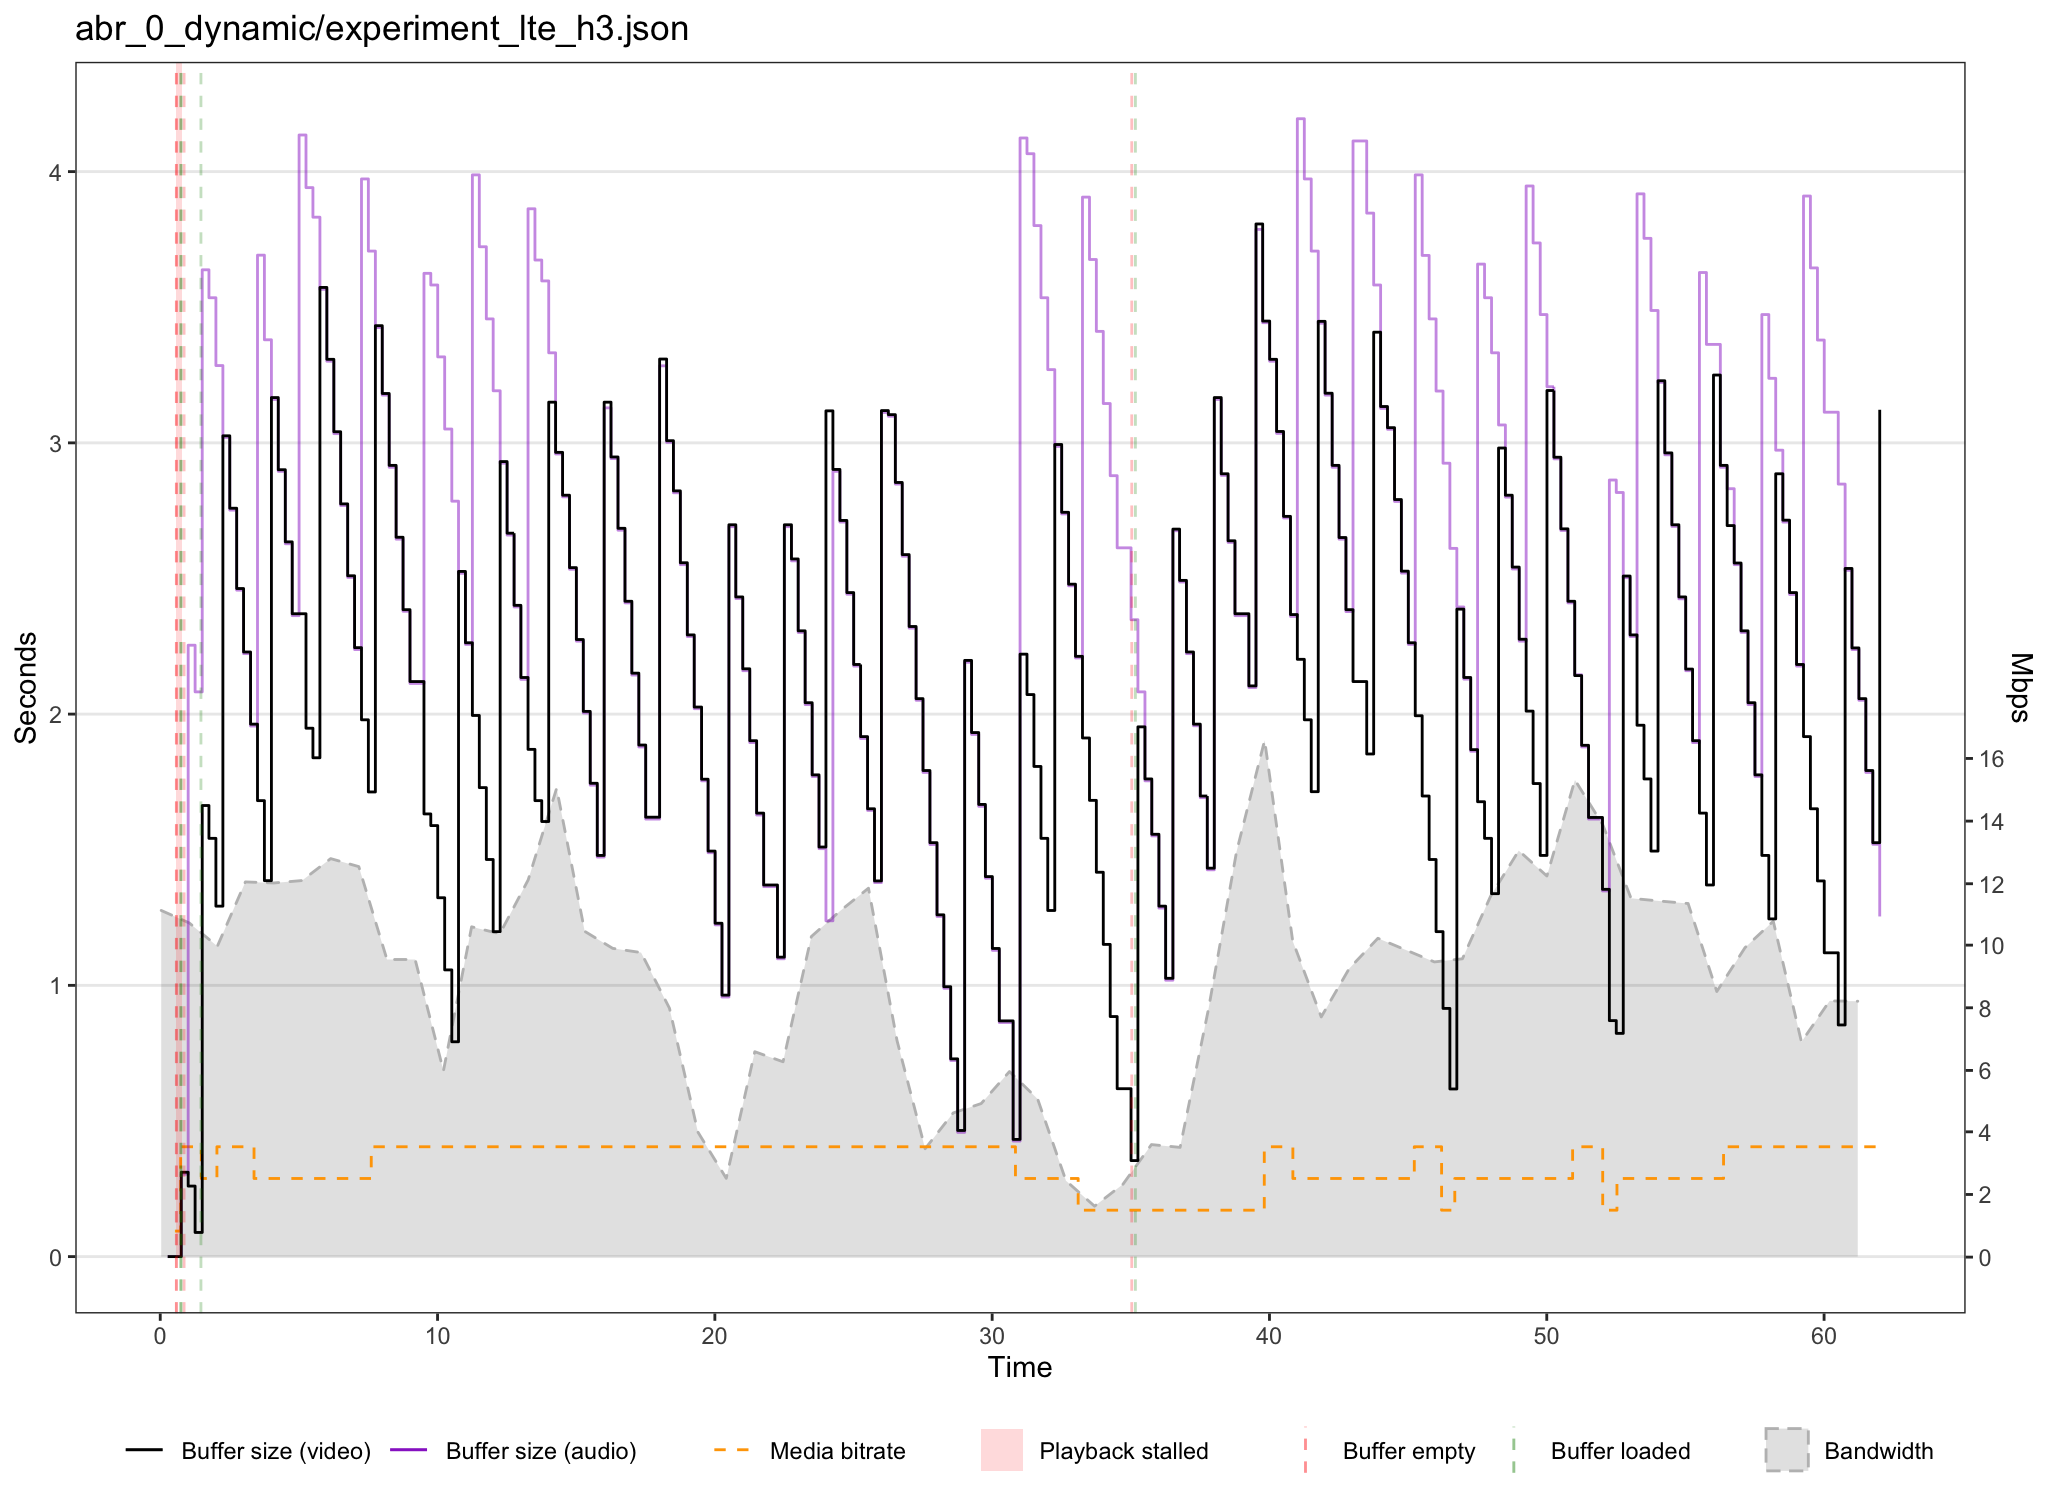
\includegraphics[width=0.9\textwidth]{res/eval_abr_dash_dynamic.png}
    \caption{Caption}
    \label{fig:eval_abr_dashjs}
\end{figure}

There is, however, an evident disadvantage to this aggressive approach, which can be seen between second 40 and second 60 in the plot. The bandwidth is always above 8 Mbps in that interval of the experiment, and thus there should be more than enough bandwidth to keep the stream at the highest quality and bitrate (3.5 Mbps).

Instead, what we observe is that the adaption algorithm keeps switching quality in a way that does not seem to make much sense. At second 40, the bitrate is raised to 3.5 Mbps but almost immediately switched down to 2.5 Mbps. The algorithm then tries to raise the bitrate again and immediately falls to 1.5 Mbps. This oscillating pattern is repeated a few times until the experiment is over.

We observed that this behavior is consistent between different runs of the same experiment and is therefore something that should be investigated.

% TODO: try both dash and hls with hspa+

\subsubsection{Other network patterns and experiments with hls.js}
\label{sec:eval/abr/hls}

To find a situation where the adaption algorithm does not behave well and leads to playback stalls, we relied on new network patterns inspired by Twitch's dataset for low-latency scenarios, introduced in \ref{sec:eval/testbed/network/patterns}. Specifically, for this analysis we will take into consideration the \texttt{spike} pattern, which contains an abrupt drop in bandwidth that lasts for a few seconds. The duration of the experiments based on this pattern is about 30 seconds.

At this point of the analysis, we also had a complete implementation of the integration with hls.js in the testbed, and therefore we run the experiments with both DASH.js and hls.js.

Figure \ref{fig:eval_abr_hls} shows the buffer health plot of an experiment run with hls.js and the \texttt{spike} network pattern over HTTP/3. As can be seen, when the bandwidth suddenly drops from about 4 Mbps to 1 Mbps the adaption algorithm struggles to react in time, causing a couple of playback stalls and thus increasing latency. An observation we could do is that if the audio had priority over video, the playback stalls would be avoided, since they are shorter than 3 seconds.

\begin{figure}[h]
    \centering
    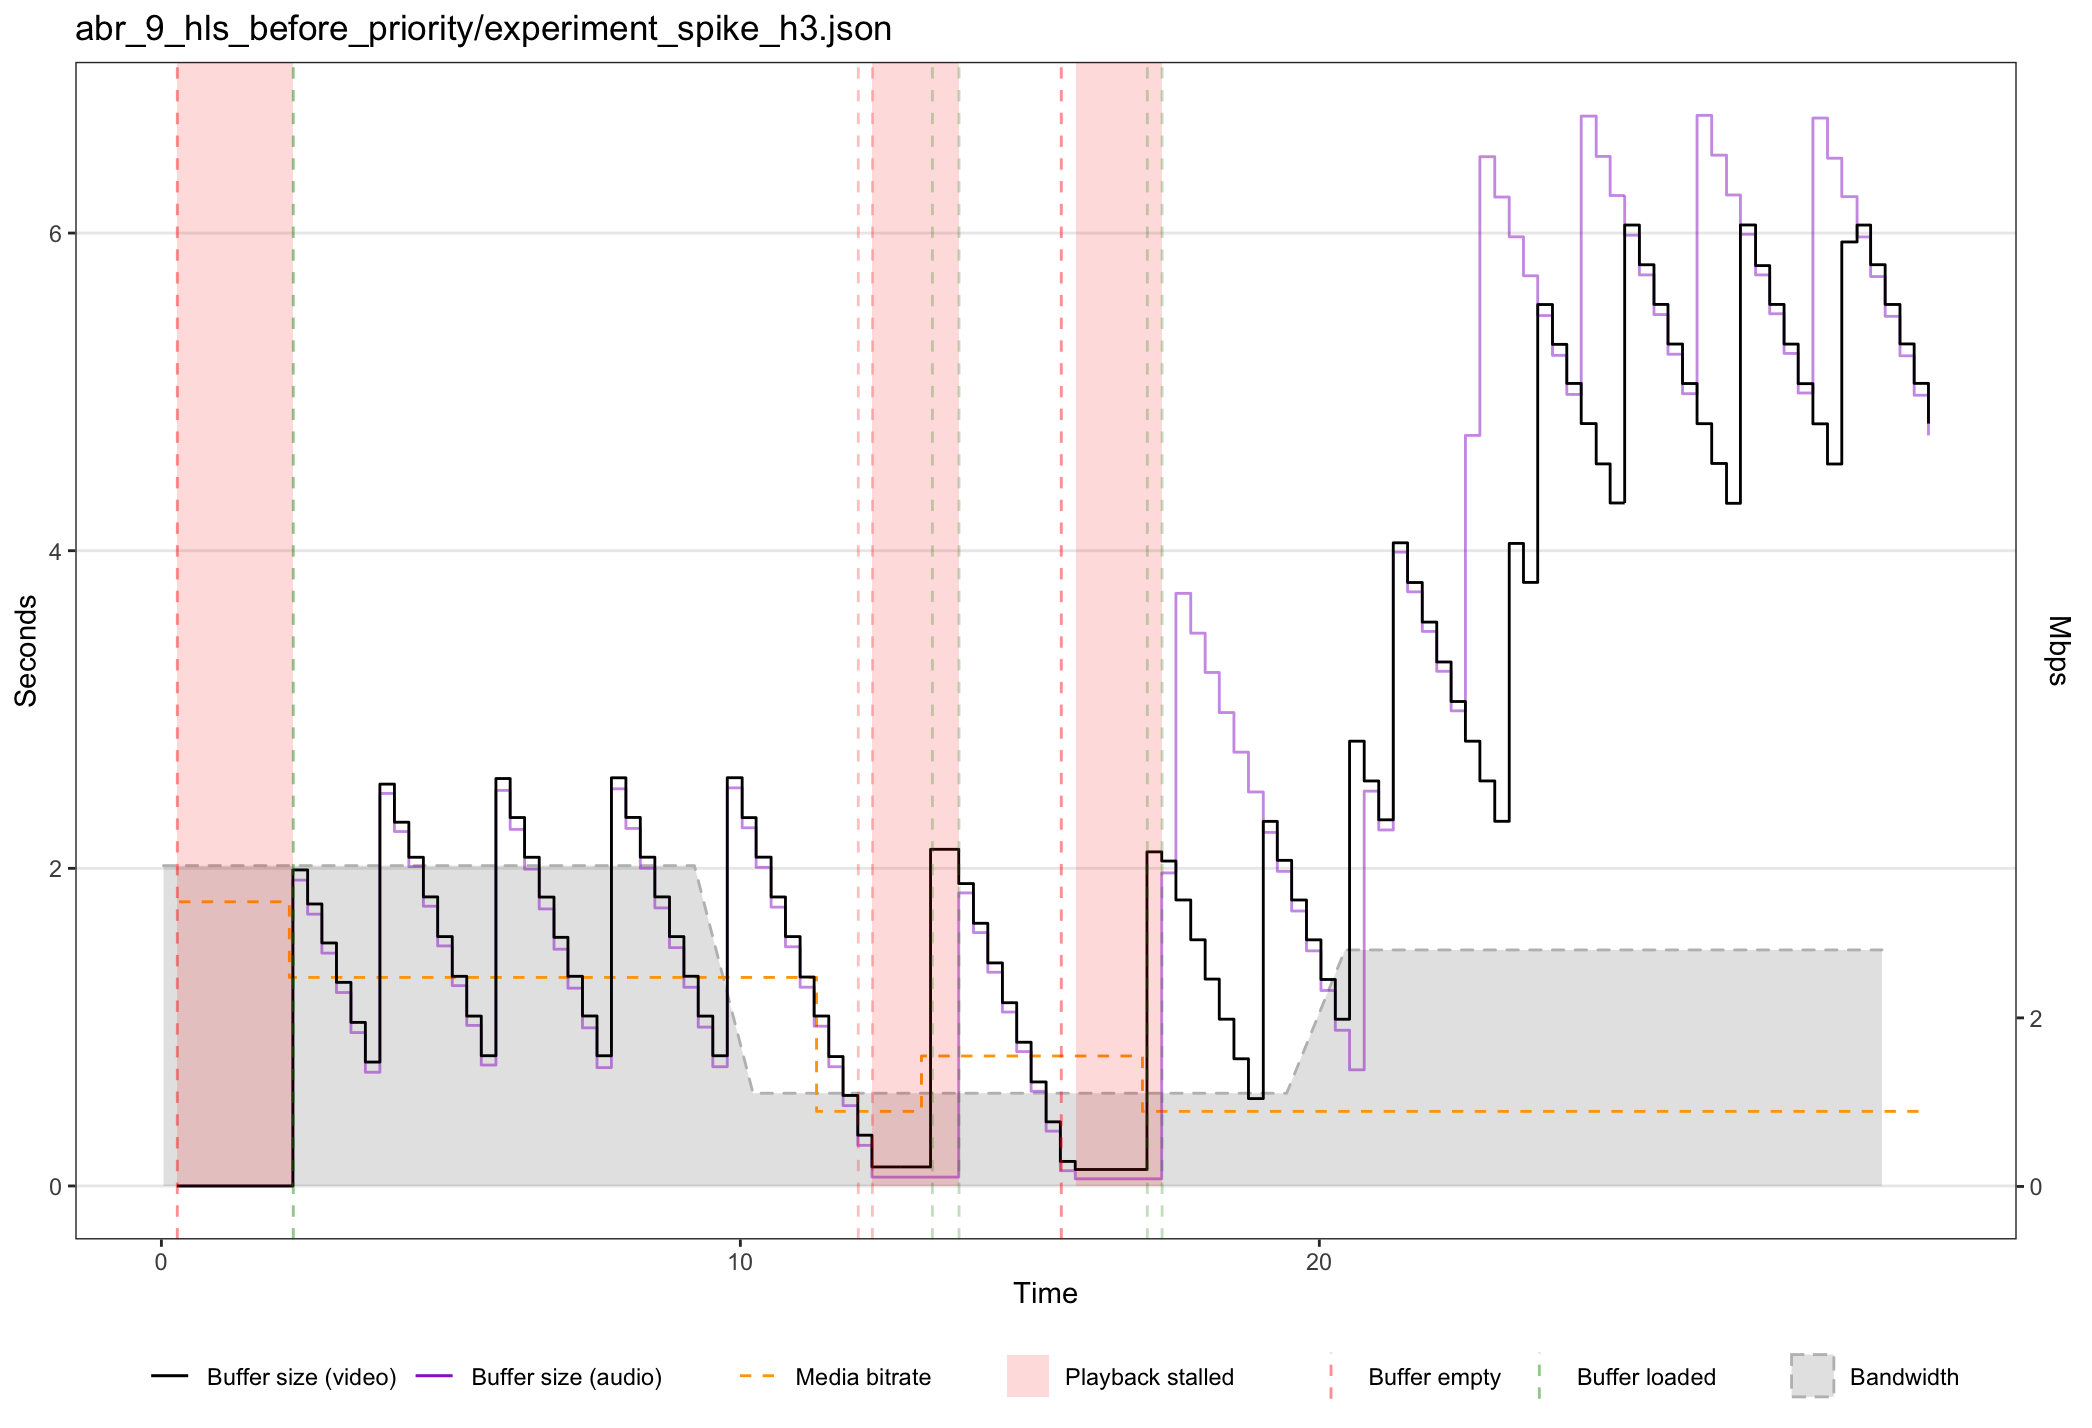
\includegraphics[width=0.9\textwidth]{res/eval_abr_spike_hls.png}
    \caption{Caption}
    \label{fig:eval_abr_hls}
\end{figure}


